\documentclass[10pt,a4paper]{article}

% ==================================================
% PACKAGES
% ==================================================
\usepackage[margin=0.62in]{geometry}
\usepackage{graphicx}
\usepackage{booktabs}
\usepackage{array}
\usepackage{float}
\usepackage{amsmath}
\usepackage{hyperref}
\usepackage{caption}
\usepackage{enumitem}
\usepackage{xcolor}
\usepackage{titlesec}
\usepackage{tcolorbox}
\usepackage{colortbl}
\usepackage{fancyhdr}
\usepackage{microtype}

% ==================================================
% COLORS
% ==================================================
\definecolor{Navy}{HTML}{17365D}
\definecolor{Blue}{HTML}{2F75B5}
\definecolor{Teal}{HTML}{008C95}
\definecolor{TealLight}{HTML}{E8F6F7}
\definecolor{Orange}{HTML}{E67E22}
\definecolor{OrangeLight}{HTML}{FFF3E8}
\definecolor{GrayLight}{HTML}{F3F5F7}
\definecolor{Gray}{HTML}{5B6573}
\definecolor{Dark}{HTML}{202733}
\definecolor{Green}{HTML}{2E7D32}
\definecolor{Red}{HTML}{C62828}

% ==================================================
% HYPERLINKS
% ==================================================
\hypersetup{
	colorlinks=true,
	linkcolor=Navy,
	urlcolor=Blue,
	citecolor=Teal
}

% ==================================================
% DOCUMENT STYLE
% ==================================================
\setlength{\parindent}{0pt}
\setlength{\parskip}{4pt}

\captionsetup{
	font=small,
	labelfont=bf,
	labelsep=period
}

% ==================================================
% SECTION HEADINGS
% ==================================================
\titleformat{\section}
{\large\bfseries\color{Navy}}
{\thesection}
{0.6em}
{}
[\color{Teal}\titlerule]

\titlespacing*{\section}
{0pt}
{7pt}
{4pt}

% ==================================================
% HEADER / FOOTER
% ==================================================
\pagestyle{fancy}
\fancyhf{}

\lhead{\small\color{Gray}
	Financial News Sentiment vs. NIFTY50}

\rhead{\small\color{Gray}
	Project Report}

\cfoot{\small\color{Gray}
	\thepage}

\renewcommand{\headrulewidth}{0.4pt}
\renewcommand{\headrule}{\hbox to\headwidth{
		\color{Teal}\leaders\hrule height \headrulewidth\hfill}}

% ==================================================
% CUSTOM BOXES
% ==================================================

\newtcolorbox{keybox}{
	colback=TealLight,
	colframe=Teal,
	boxrule=0.8pt,
	arc=3pt,
	left=7pt,
	right=7pt,
	top=5pt,
	bottom=5pt
}

\newtcolorbox{resultbox}{
	colback=OrangeLight,
	colframe=Orange,
	boxrule=0.8pt,
	arc=3pt,
	left=7pt,
	right=7pt,
	top=5pt,
	bottom=5pt
}

% ==================================================
% DOCUMENT
% ==================================================
\begin{document}
	
	% ==================================================
	% TITLE
	% ==================================================
	
	\begin{center}
		
		\vspace*{-0.25cm}
		
		{\Large\bfseries\color{Navy}
			Financial News Sentiment vs. NIFTY50 Movement}
		
		\vspace{3pt}
		
		{\normalsize\color{Teal}
			Project Report}
		
		\vspace{5pt}
		
		{\small\color{Gray}
			\textbf{}}
		
		\vspace{5pt}
		
		{\color{Orange}\rule{0.85\linewidth}{1.2pt}}
		
	\end{center}
	
	% ==================================================
	\section{Project Overview}
	% ==================================================
	
	This project investigates whether sentiment expressed in financial
	news headlines can help explain or predict the direction of the NIFTY50
	index. The analysis combines financial news data with historical NIFTY50
	market data and develops two sentiment-analysis approaches: a
	rule-based financial sentiment method and the pretrained FinBERT
	financial-language model.
	
	The complete workflow includes data cleaning, date alignment, news
	aggregation, rule-based sentiment scoring, FinBERT sentiment extraction,
	feature engineering, exploratory analysis, time-aware machine learning,
	model comparison, prediction-error analysis, and a simple backtest.
	
	The central objective is to determine whether financial-news sentiment,
	when combined with recent market information, provides a useful signal
	for predicting the next-day direction of the NIFTY50.
	
	% ==================================================
	% KEY RESULTS BOX
	% ==================================================
	
	\begin{keybox}
		\textbf{\color{Navy}Key Results}
		
		\smallskip
		
		\begin{tabular}{@{}lll@{}}
			\textbf{Merged observations} & 132 & \\
			\textbf{Usable ML observations} & 125 & \\
			\textbf{Training / Test split} & 100 / 25 & \\
			\textbf{Rule-based same-day accuracy} & 59.0\% & \\
			\textbf{Best original test accuracy} & 44.0\% & \\
			\textbf{Best FinBERT test accuracy} & 36.0\% & \\
			\textbf{Best CV accuracy} & 51.25\% & \\
			\textbf{Rule-Based vs. FinBERT correlation} & 0.407 & \\
			\textbf{Buy-and-Hold return} & -0.64\% & \\
			\textbf{Model strategy return} & -0.77\% &
		\end{tabular}
	\end{keybox}
	
	% ==================================================
	\section{Changes and Contributions}
	% ==================================================
	
	The project was extended beyond the original rule-based sentiment
	pipeline by introducing FinBERT and a second machine-learning feature
	set.
	
	The main changes and contributions were:
	
	\begin{itemize}[
		leftmargin=*,
		itemsep=1pt,
		topsep=2pt
		]
		
		\item Cleaned and standardized the financial news and NIFTY50
		datasets.
		
		\item Aligned financial news and market observations using trading
		dates.
		
		\item Grouped multiple news headlines occurring on the same date.
		
		\item Implemented a financial rule-based sentiment scoring system
		using positive and negative financial vocabulary.
		
		\item Constructed a same-day sentiment-based prediction rule and
		evaluated its accuracy.
		
		\item Corrected the machine-learning target so that models predict
		the \textbf{next trading day's} NIFTY50 direction.
		
		\item Created rolling sentiment features including three-day and
		seven-day moving averages and short-term sentiment variability.
		
		\item Created market features including lagged movement, volume
		change, and high-low spread.
		
		\item Added FinBERT using the \texttt{ProsusAI/finbert} pretrained
		financial-language model.
		
		\item Converted FinBERT predictions into numerical sentiment scores
		using confidence-weighted positive and negative values.
		
		\item Created FinBERT rolling features:
		\texttt{finbert\_ma3}, \texttt{finbert\_ma7}, and
		\texttt{finbert\_std3}.
		
		\item Compared rule-based sentiment directly with FinBERT sentiment.
		
		\item Measured the correlation between the two sentiment approaches.
		
		\item Trained Logistic Regression and Random Forest models using the
		FinBERT-based feature set.
		
		\item Compared the original models and FinBERT-based models on the
		same chronological test period.
		
		\item Used a chronological train/test split to avoid future-data
		leakage.
		
		\item Performed Random Forest hyperparameter tuning using
		TimeSeriesSplit cross-validation.
		
		\item Evaluated predictions using accuracy, classification reports,
		and confusion matrices.
		
		\item Analyzed Random Forest feature importance.
		
		\item Compared a model-based trading strategy against buy-and-hold.
		
	\end{itemize}
	
	% ==================================================
	\section{Data and Feature Engineering}
	% ==================================================
	
	The financial news dataset contains multiple headlines per trading day,
	while the NIFTY50 dataset contains daily OHLC and trading information.
	The two datasets were cleaned and aligned using their trading dates.
	
	After merging the datasets, 132 observations were available. Following
	the creation of rolling features and removal of rows containing
	unavailable values, 125 observations were used for the final
	machine-learning experiments.
	
	The original feature set consisted of eight features:
	
	\begin{center}
		\small
		\rowcolors{1}{GrayLight}{white}
		\begin{tabular}{>{\ttfamily}llll}
			sentiment\_score &
			sentiment\_ma3 &
			sentiment\_ma7 &
			sentiment\_std3 \\
			
			movement\_lag1 &
			movement\_lag2 &
			volume\_change &
			high\_low\_spread
		\end{tabular}
	\end{center}
	
	The FinBERT feature set replaced the original sentiment features with
	four FinBERT-derived variables while retaining the market features:
	
	\begin{center}
		\small
		\rowcolors{1}{GrayLight}{white}
		\begin{tabular}{>{\ttfamily}llll}
			finbert\_score &
			finbert\_ma3 &
			finbert\_ma7 &
			finbert\_std3 \\
			
			movement\_lag1 &
			movement\_lag2 &
			volume\_change &
			high\_low\_spread
		\end{tabular}
	\end{center}
	
	The target variable represents whether the NIFTY50 moves upward on the
	following trading day. The data was sorted chronologically before the
	target was shifted.
	
	The final machine-learning dataset contained 125 observations, with
	100 observations used for training and 25 observations reserved for the
	final test period.
	
	\begin{resultbox}
		\textbf{\color{Orange}Time-aware evaluation:}
		The first 100 observations were used for training, while the final
		25 observations were kept completely unseen for final evaluation.
		This chronological design prevents future observations from being
		mixed into the training data.
	\end{resultbox}
	
	% ==================================================
	\section{Rule-Based Sentiment Analysis}
	% ==================================================
	
	The original sentiment system assigns scores to financial news
	headlines using a manually constructed financial vocabulary. Positive
	terms increase the score while negative terms decrease it.
	
	The sentiment score is then converted into a simple prediction:
	
	\begin{itemize}[leftmargin=*]
		\item Positive score $\rightarrow$ UP
		\item Negative score $\rightarrow$ DOWN
		\item Zero score $\rightarrow$ NEUTRAL
	\end{itemize}
	
	For the binary prediction used in evaluation, positive sentiment was
	mapped to an upward movement and non-positive sentiment to a downward
	movement.
	
	The rule-based approach achieved a same-day prediction accuracy of
	approximately 59.0\%.
	
	However, this result must not be interpreted as a next-day forecasting
	result. The rule-based sentiment score and the original target are
	calculated from the same trading day. Therefore, the 59.0\% accuracy
	primarily reflects same-day co-movement between news sentiment and
	market movement rather than genuine future prediction.
	
	This distinction motivated the next-day target used in the machine
	learning section.
	
	% ==================================================
	\section{Original Exploratory Data Analysis}
	% ==================================================
	
	The original rule-based sentiment distribution is shown in
	Figure~\ref{fig:histogram}.
	
	\begin{figure}[H]
		\centering
		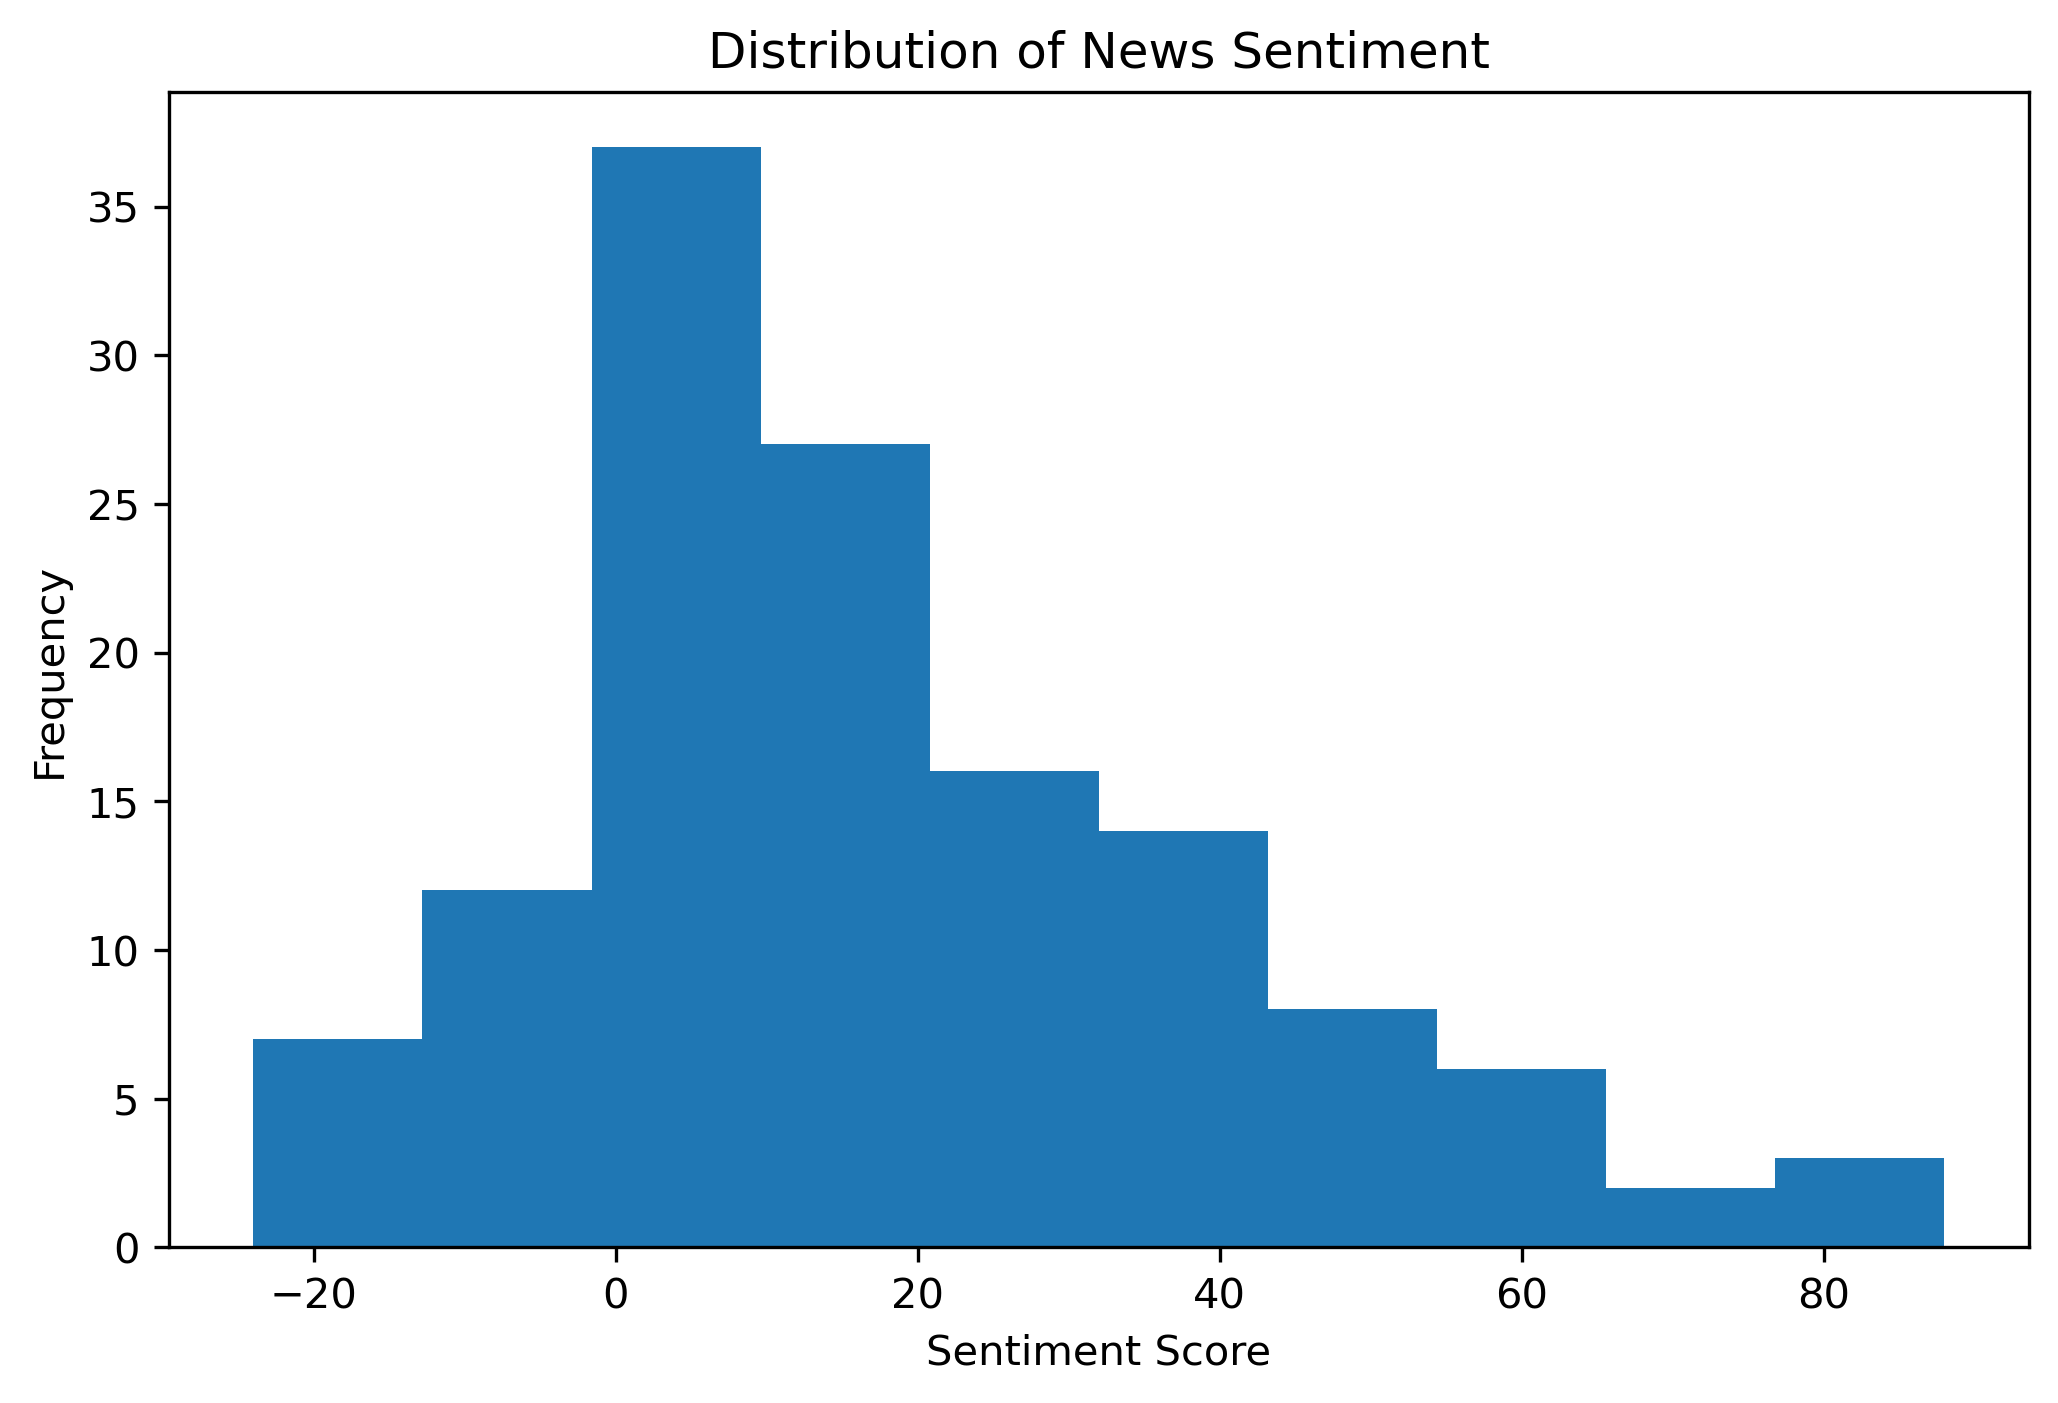
\includegraphics[
		width=0.72\linewidth
		]{../plots/histogram.png}
		
		\caption{
			Distribution of the original rule-based financial-news
			sentiment scores.
		}
		
		\label{fig:histogram}
	\end{figure}
	
	The average rule-based sentiment by market direction is shown in
	Figure~\ref{fig:barplot}.
	
	\begin{figure}[H]
		\centering
		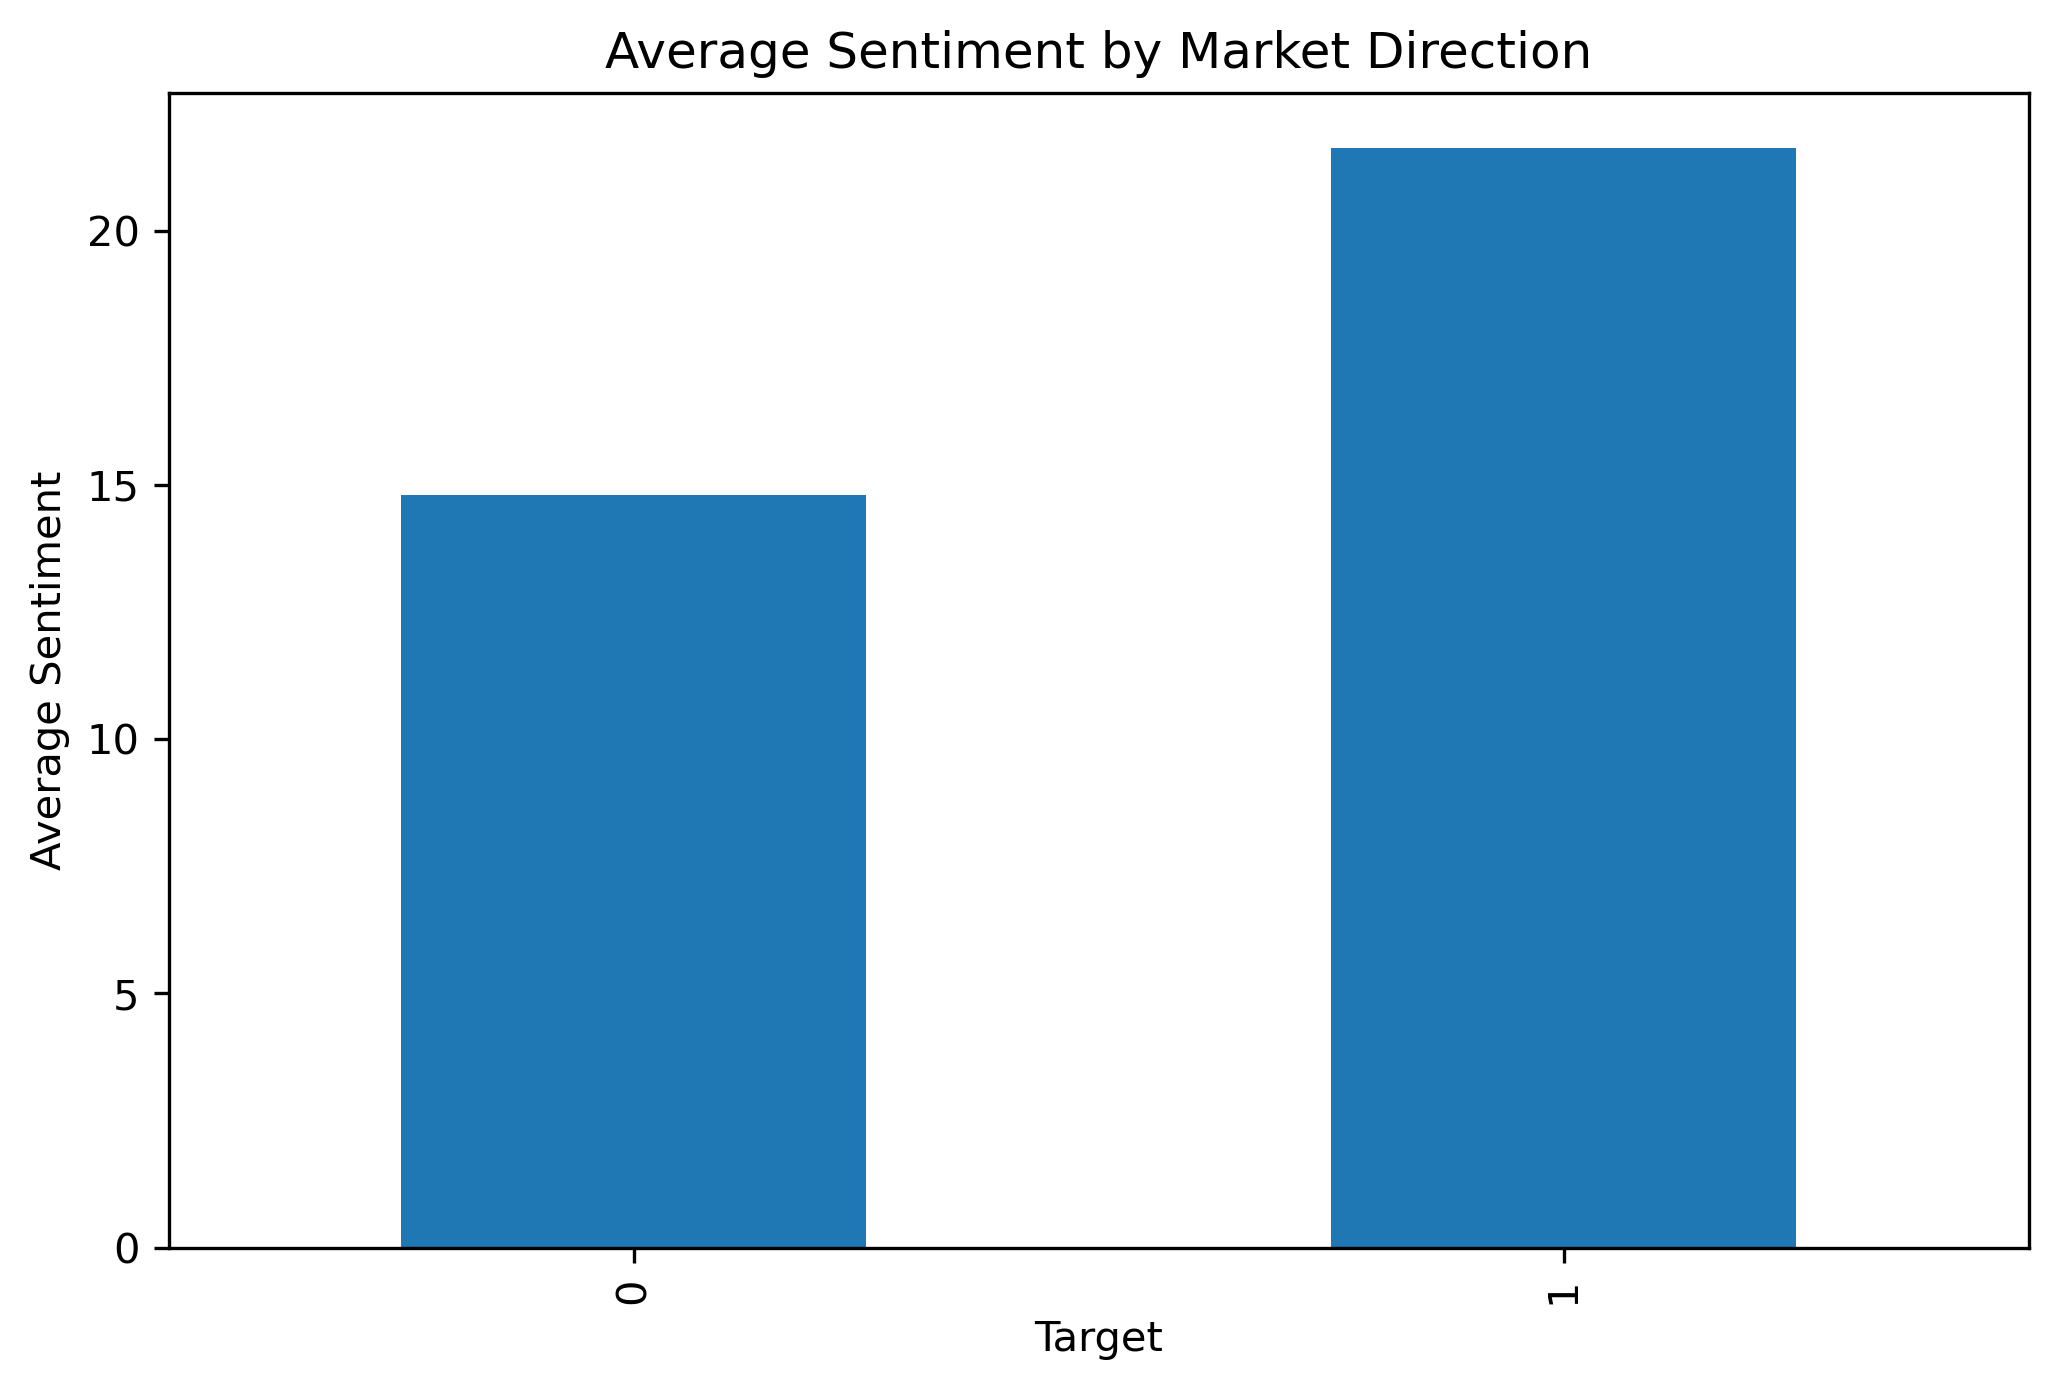
\includegraphics[
		width=0.72\linewidth
		]{../plots/barplot.png}
		
		\caption{
			Average rule-based sentiment by NIFTY50 market direction.
		}
		
		\label{fig:barplot}
	\end{figure}
	
	The relationship between rule-based sentiment and same-day market
	movement is shown in Figure~\ref{fig:scatterplot}.
	
	\begin{figure}[H]
		\centering
		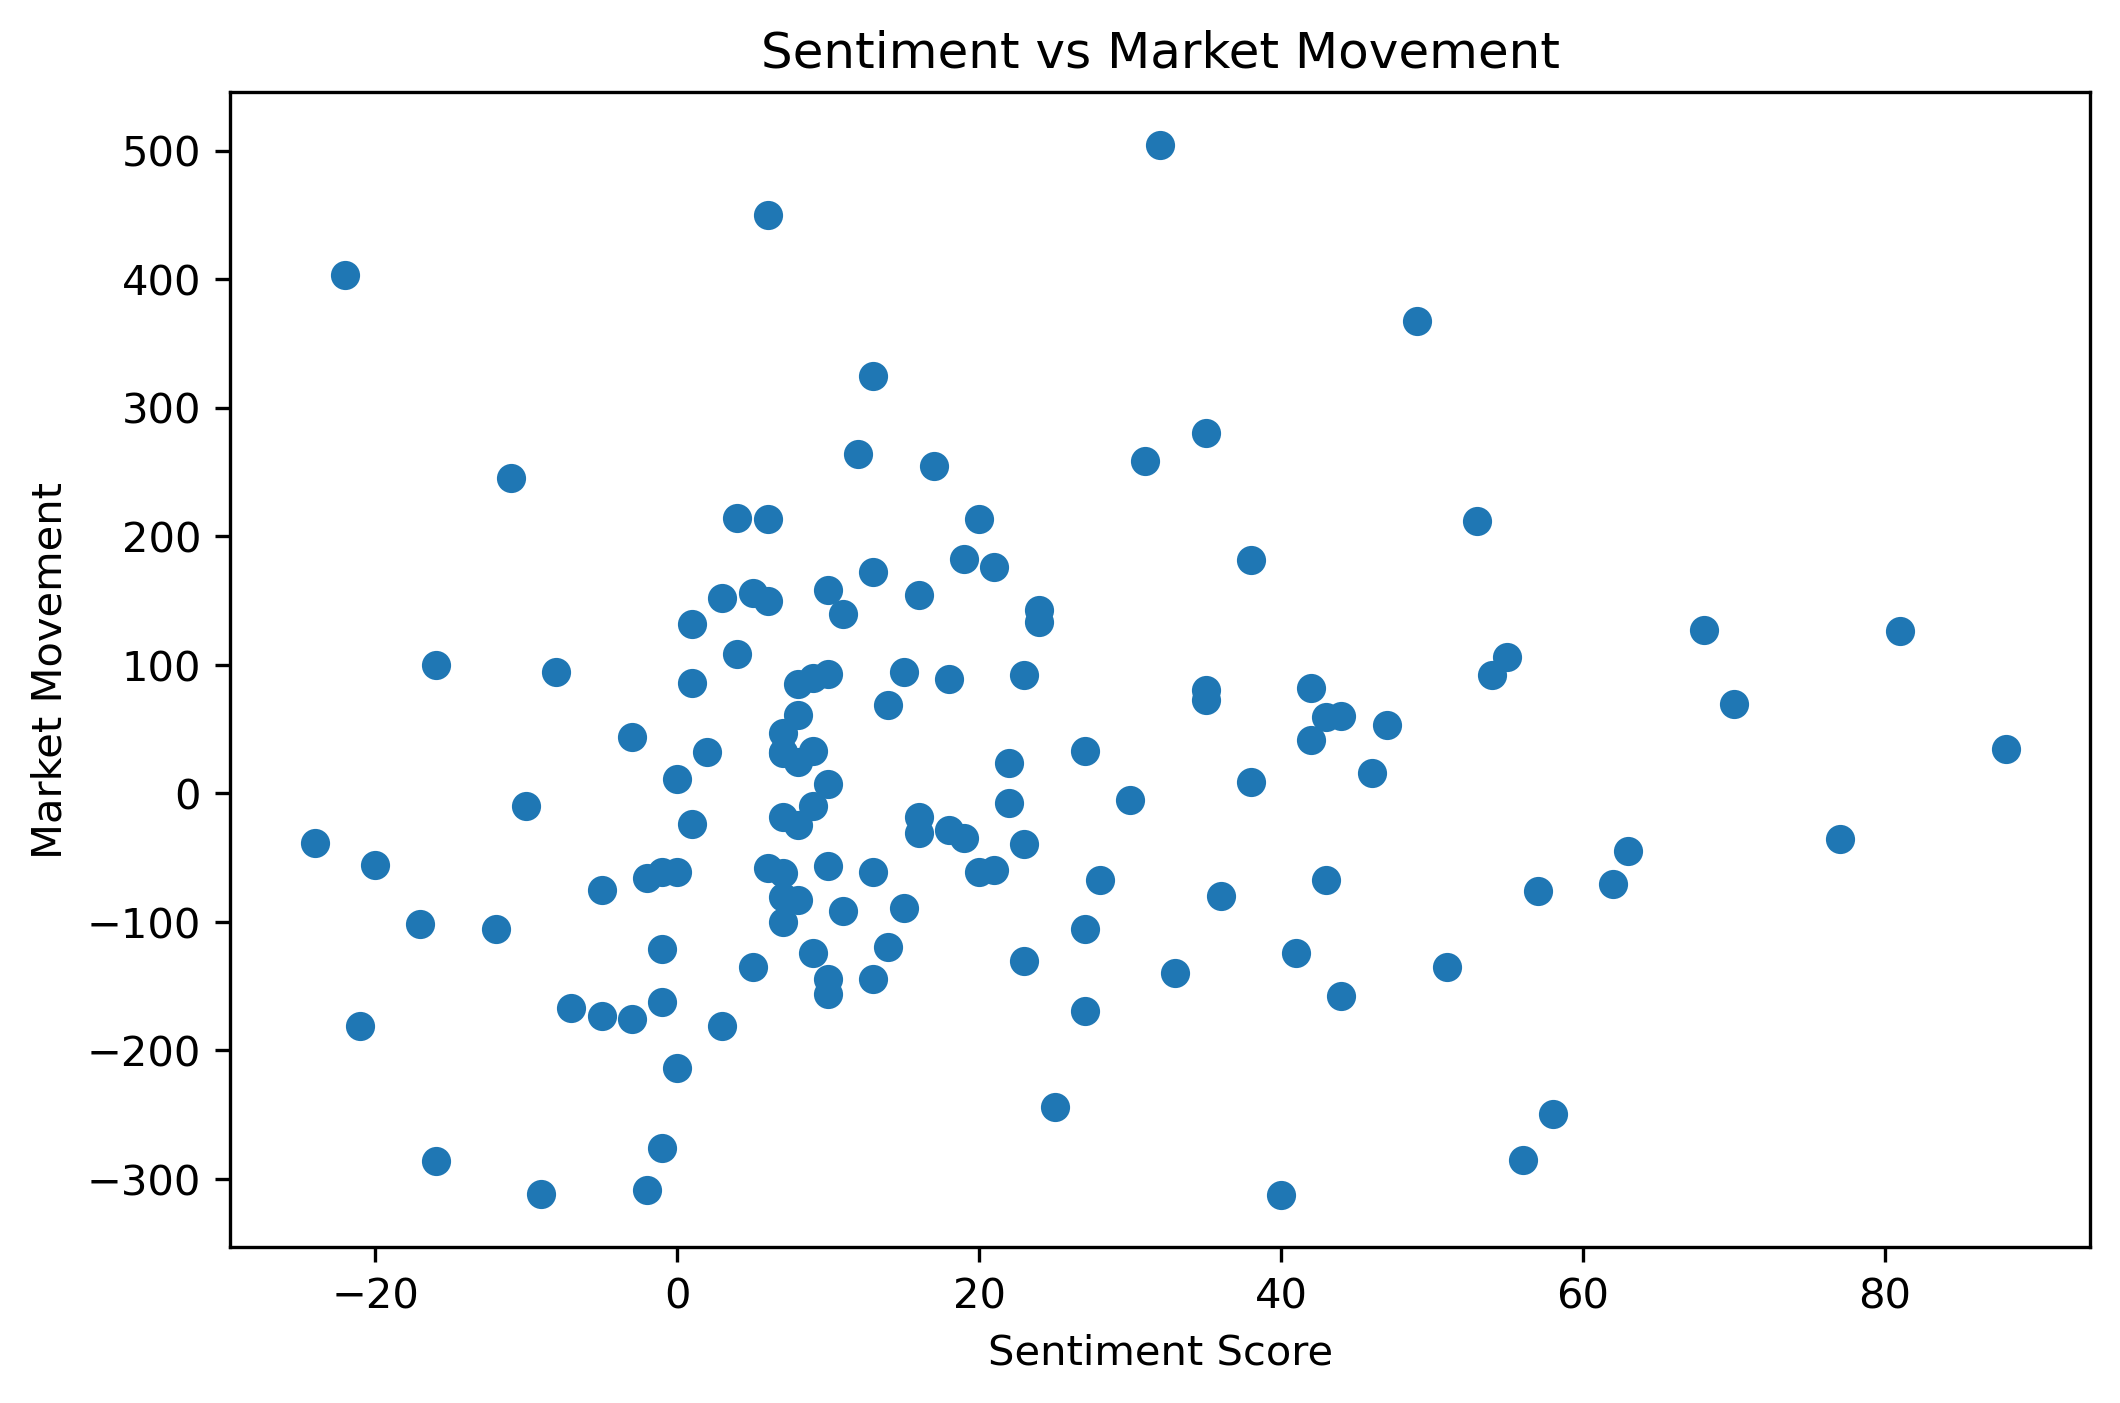
\includegraphics[
		width=0.72\linewidth
		]{../plots/scatterplot.png}
		
		\caption{
			Relationship between rule-based sentiment and same-day
			NIFTY50 market movement.
		}
		
		\label{fig:scatterplot}
	\end{figure}
	
	These plots provide useful exploratory evidence that financial-news
	sentiment and market movement can co-move. They should not, however, be
	interpreted as evidence of reliable next-day prediction.
	
	% ==================================================
	\section{FinBERT Sentiment Analysis}
	% ==================================================
	
	To extend the original rule-based approach, the project introduced
	FinBERT, a pretrained language model designed for financial text.
	
	Each headline was processed using FinBERT to obtain:
	
	\begin{itemize}[leftmargin=*]
		\item a sentiment label: positive, neutral, or negative;
		\item a confidence score;
		\item a numerical sentiment score.
	\end{itemize}
	
	The numerical FinBERT sentiment score was constructed as follows:
	
	\[
	S_{\mathrm{FinBERT}} =
	\begin{cases}
		+C, & \text{if the label is positive},\\
		-C, & \text{if the label is negative},\\
		0, & \text{if the label is neutral},
	\end{cases}
	\]
	
	where $C$ represents the model confidence.
	
	This produces a continuous sentiment score that preserves both the
	direction and confidence of the FinBERT prediction.
	
	% ==================================================
	\subsection{FinBERT Sentiment Distribution}
	% ==================================================
	
	The distribution of FinBERT sentiment labels is shown below.
	
	\begin{figure}[H]
		\centering
		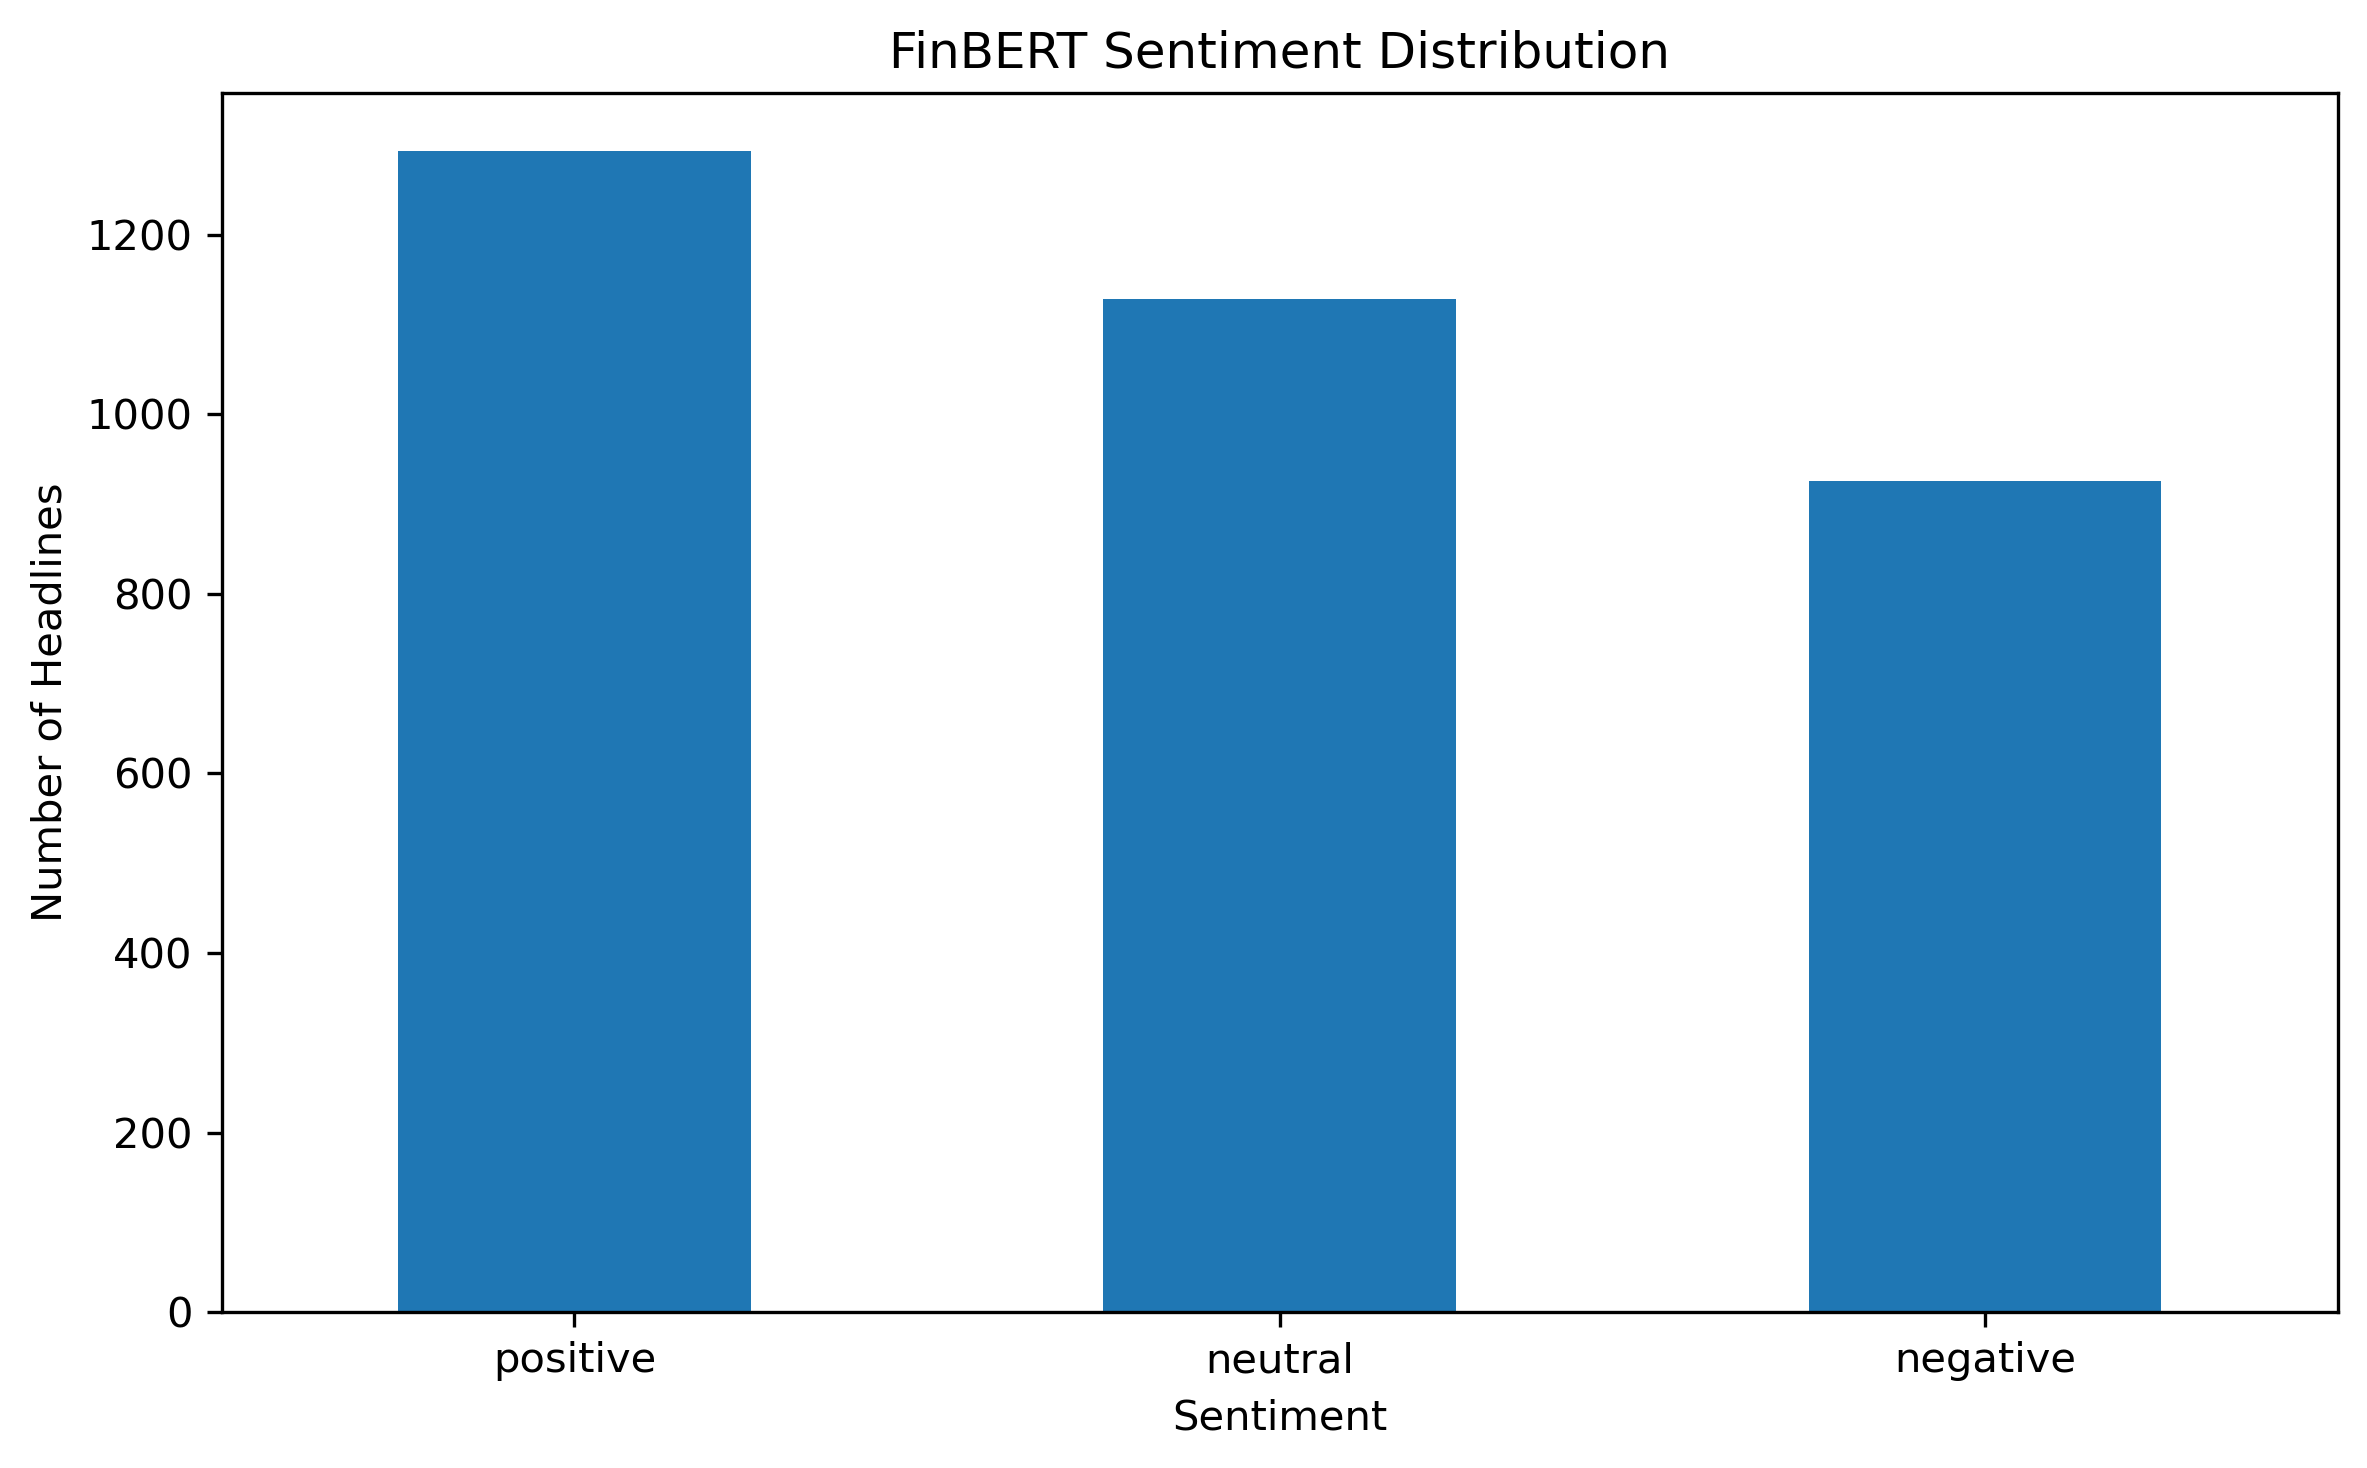
\includegraphics[
		width=0.72\linewidth
		]{../plots/finbert_sentiment_distribution.png}
		
		\caption{
			Distribution of FinBERT sentiment labels across financial-news
			headlines.
		}
		
		\label{fig:finbert_distribution}
	\end{figure}
	
	The FinBERT output provides a model-based alternative to the manually
	constructed rule-based vocabulary. Unlike the rule-based approach,
	FinBERT evaluates the linguistic context of each headline using a
	pretrained financial-language model.
	
	% ==================================================
	\subsection{Rule-Based Sentiment vs. FinBERT}
	% ==================================================
	
	The two sentiment approaches were directly compared using their
	numerical scores.
	
	\begin{figure}[H]
		\centering
		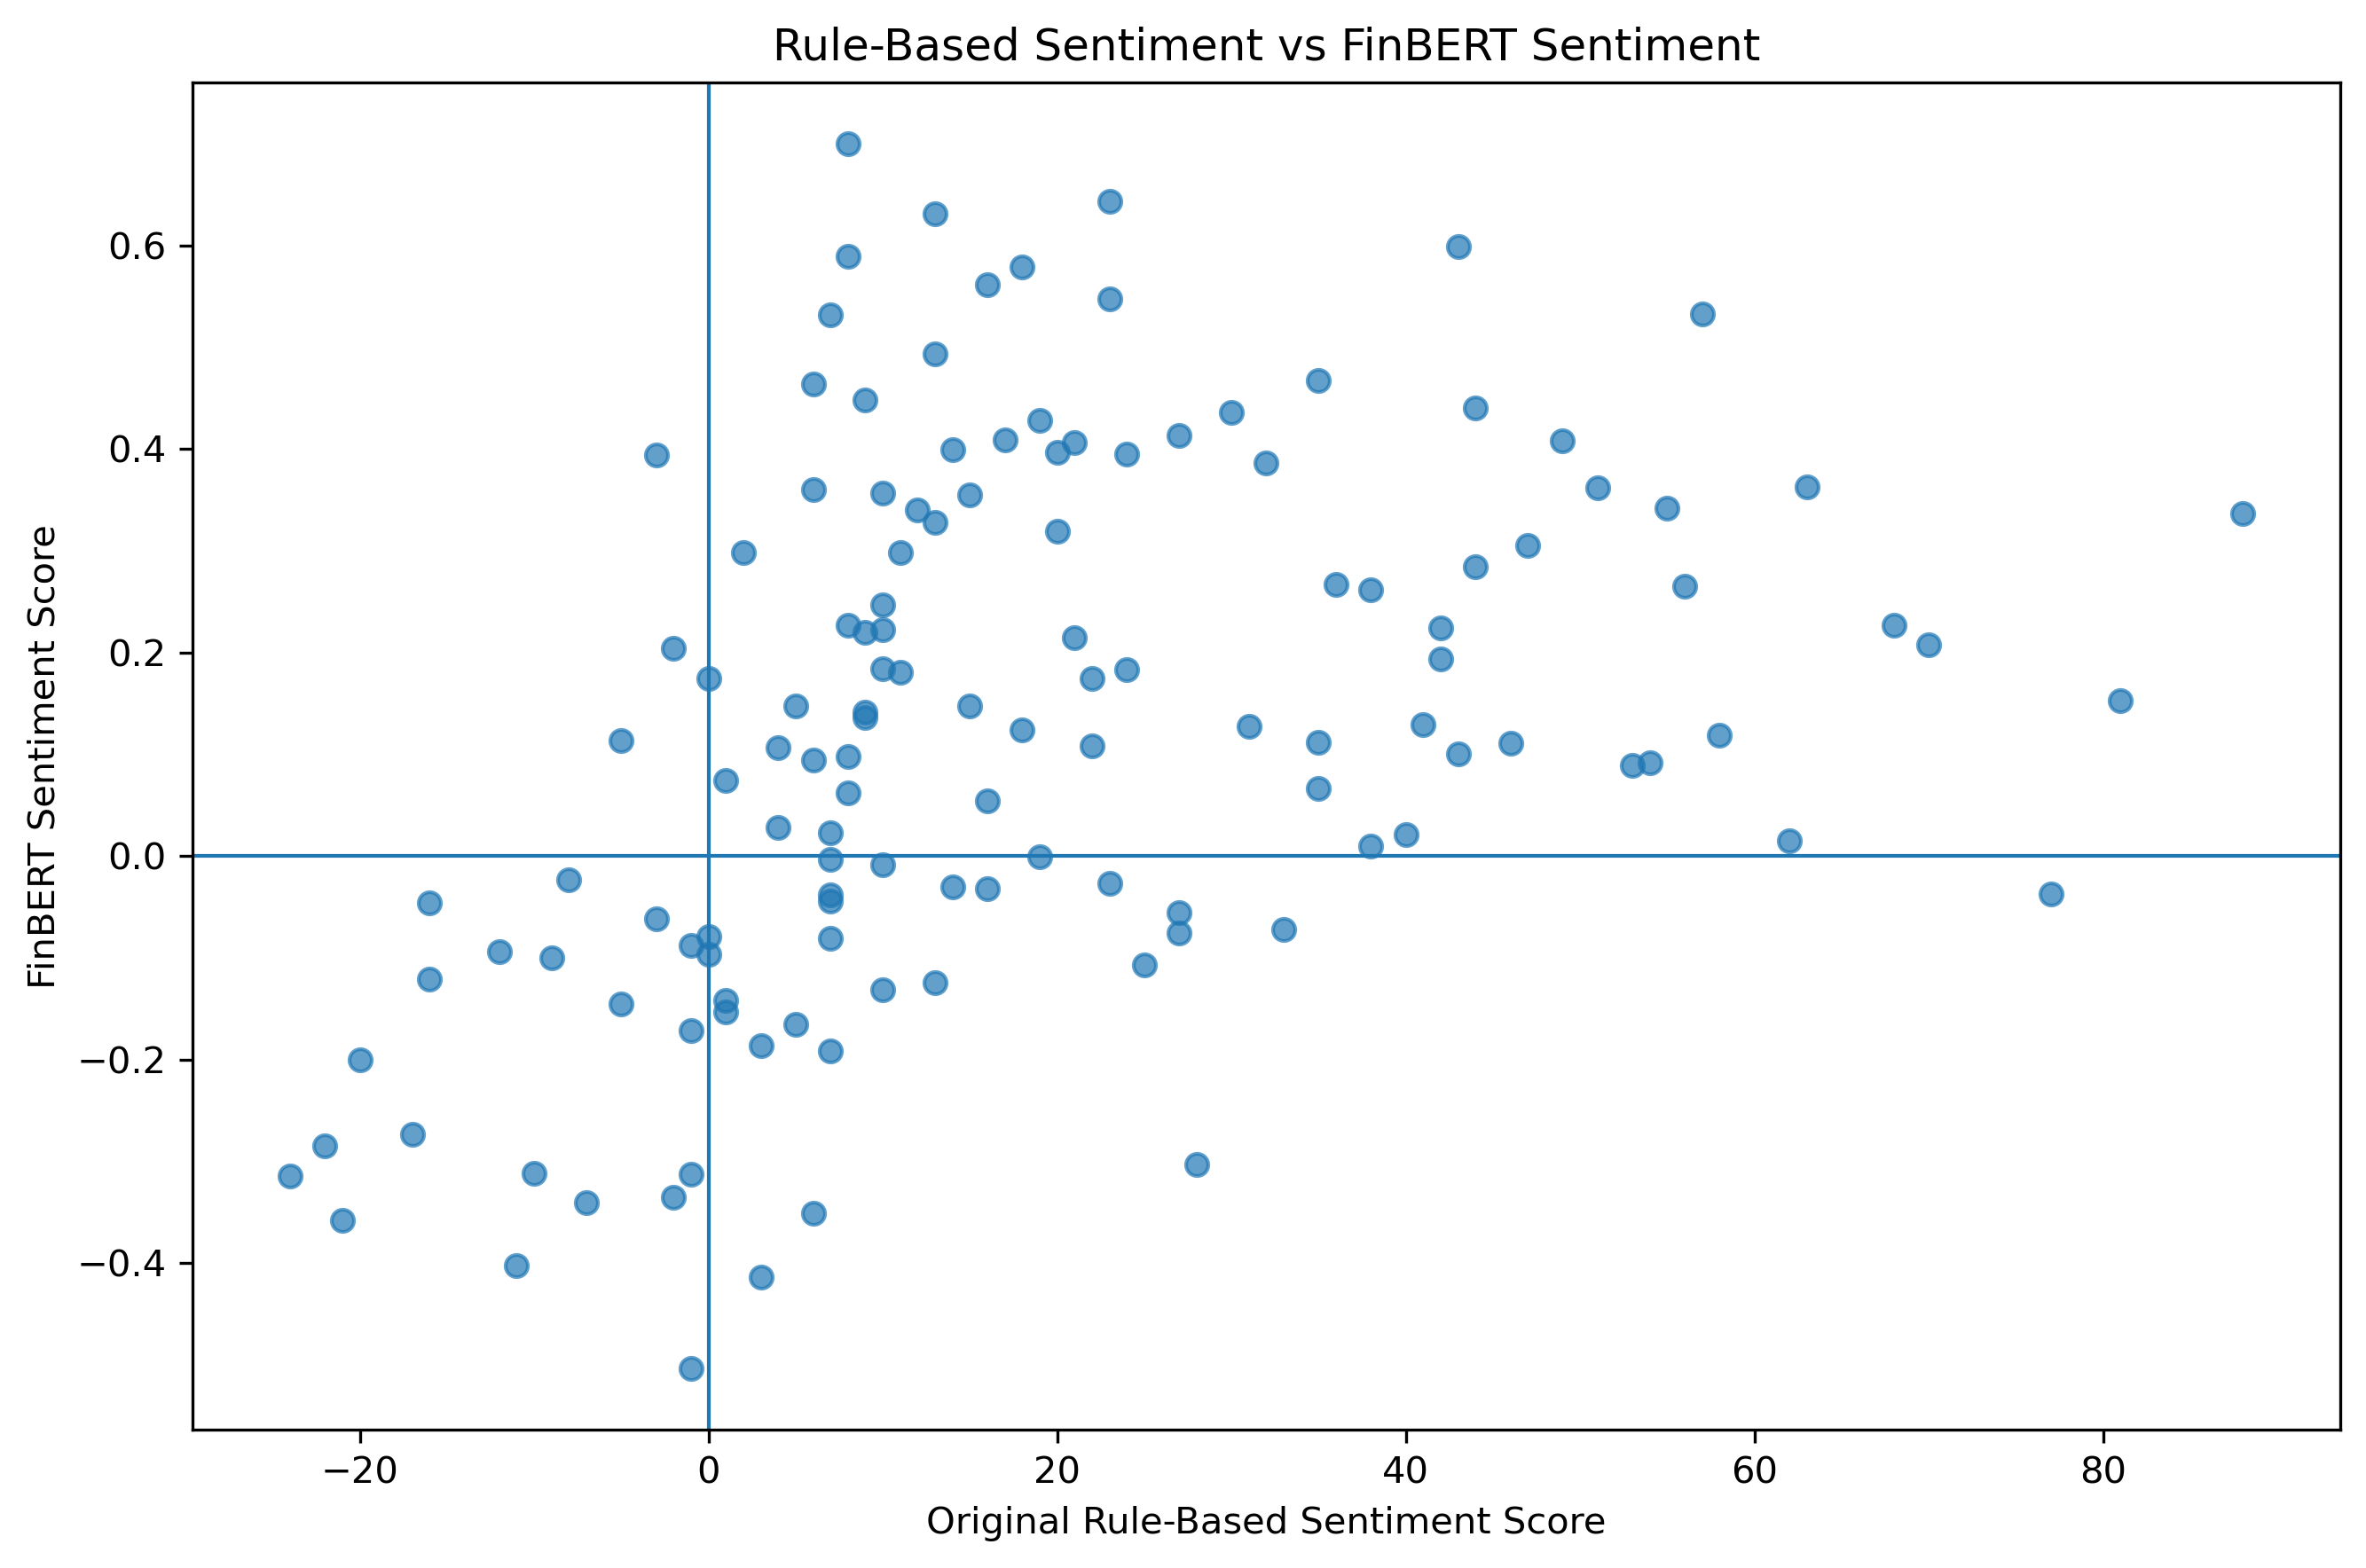
\includegraphics[
		width=0.72\linewidth
		]{../plots/rule_based_vs_finbert.png}
		
		\caption{
			Comparison between the original rule-based sentiment score and
			the FinBERT sentiment score.
		}
		
		\label{fig:rulefinbert}
	\end{figure}
	
	The correlation between the two sentiment measures was approximately
	0.407.
	
	This represents a moderate positive relationship: the two methods
	often identify broadly similar sentiment direction, but they are far
	from identical. This is expected because the rule-based method relies
	on manually specified financial vocabulary, whereas FinBERT uses a
	pretrained language representation.
	
	The comparison therefore demonstrates that FinBERT provides additional
	information rather than simply reproducing the original rule-based
	score.
	
	\begin{resultbox}
		\textbf{\color{Orange}Important interpretation:}
		A correlation of 0.407 indicates meaningful overlap between the two
		sentiment measures, but it is not sufficiently high to consider
		them equivalent. The methods capture different aspects of headline
		sentiment.
	\end{resultbox}
	
	% ==================================================
	\section{Machine Learning Analysis}
	% ==================================================
	
	The machine-learning task was framed as a next-day classification
	problem. The target was shifted by one trading day so that features
	available on day $t$ were used to predict the market direction on
	day $t+1$.
	
	The original models evaluated were:
	
	\begin{itemize}[leftmargin=*]
		\item Logistic Regression
		\item Random Forest
		\item XGBoost
		\item Tuned Random Forest
	\end{itemize}
	
	The FinBERT feature set was subsequently evaluated using:
	
	\begin{itemize}[leftmargin=*]
		\item FinBERT Logistic Regression
		\item FinBERT Random Forest
	\end{itemize}
	
	A majority-class classifier was included as the baseline.
	
	% ==================================================
	\subsection{Original Model Results}
	% ==================================================
	
	\begin{table}[H]
		\centering
		\caption{Original model performance on the held-out test period.}
		
		\vspace{2pt}
		
		\rowcolors{2}{GrayLight}{white}
		\begin{tabular}{>{\bfseries}l c}
			\toprule
			\rowcolor{Navy}
			\color{white}\textbf{Model} &
			\color{white}\textbf{Accuracy} \\
			\midrule
			Majority Baseline & 44.0\% \\
			Logistic Regression & 44.0\% \\
			Random Forest & 44.0\% \\
			XGBoost & 40.0\% \\
			Tuned Random Forest & \textbf{44.0\%} \\
			\bottomrule
		\end{tabular}
	\end{table}
	
	The original Logistic Regression and Random Forest models matched the
	44.0\% majority baseline. XGBoost performed slightly worse at 40.0\%.
	
	The tuned Random Forest selected the following parameters:
	
	\begin{center}
		\small
		\begin{tabular}{>{\ttfamily}l l}
			\toprule
			n\_estimators & 100 \\
			max\_depth & 3 \\
			min\_samples\_leaf & 20 \\
			\bottomrule
		\end{tabular}
	\end{center}
	
	The best time-series cross-validation accuracy was 51.25\%, but the
	accuracy on the untouched test period remained 44.0\%.
	
	Therefore, hyperparameter tuning improved the cross-validation
	selection process but did not improve final out-of-sample accuracy.
	
	% ==================================================
	\subsection{FinBERT Model Results}
	% ==================================================
	
	The FinBERT-based machine-learning dataset used the four FinBERT
	sentiment features together with four market features.
	
	The FinBERT model results were:
	
	\begin{table}[H]
		\centering
		\caption{FinBERT-based model performance on the held-out test period.}
		
		\vspace{2pt}
		
		\rowcolors{2}{GrayLight}{white}
		\begin{tabular}{>{\bfseries}l c}
			\toprule
			\rowcolor{Navy}
			\color{white}\textbf{Model} &
			\color{white}\textbf{Accuracy} \\
			\midrule
			FinBERT Logistic Regression & 36.0\% \\
			FinBERT Random Forest & 28.0\% \\
			\bottomrule
		\end{tabular}
	\end{table}
	
	The FinBERT Logistic Regression model achieved 36.0\% accuracy, while
	the FinBERT Random Forest achieved 28.0%.
	
	Therefore, replacing the original rule-based sentiment features with
	the FinBERT-derived features did not improve predictive performance
	on the final test period.
	
	% ==================================================
	\section{Final Model Comparison}
	% ==================================================
	
	The complete comparison between the original and FinBERT-based
	approaches is shown in Table~\ref{tab:allmodels}.
	
	\begin{table}[H]
		\centering
		\caption{Complete model comparison on the held-out test period.}
		\label{tab:allmodels}
		
		\vspace{2pt}
		
		\rowcolors{2}{GrayLight}{white}
		\begin{tabular}{>{\bfseries}l c}
			\toprule
			\rowcolor{Navy}
			\color{white}\textbf{Model} &
			\color{white}\textbf{Accuracy} \\
			\midrule
			Majority Baseline & 44.0\% \\
			Original Logistic Regression & 44.0\% \\
			Original Random Forest & 44.0\% \\
			Original XGBoost & 40.0\% \\
			Original Tuned Random Forest & \textbf{44.0\%} \\
			FinBERT Logistic Regression & 36.0\% \\
			FinBERT Random Forest & 28.0\% \\
			\bottomrule
		\end{tabular}
	\end{table}
	
	The complete comparison is also visualized in Figure~\ref{fig:modelcomparison}.
	
	\begin{figure}[H]
		\centering
		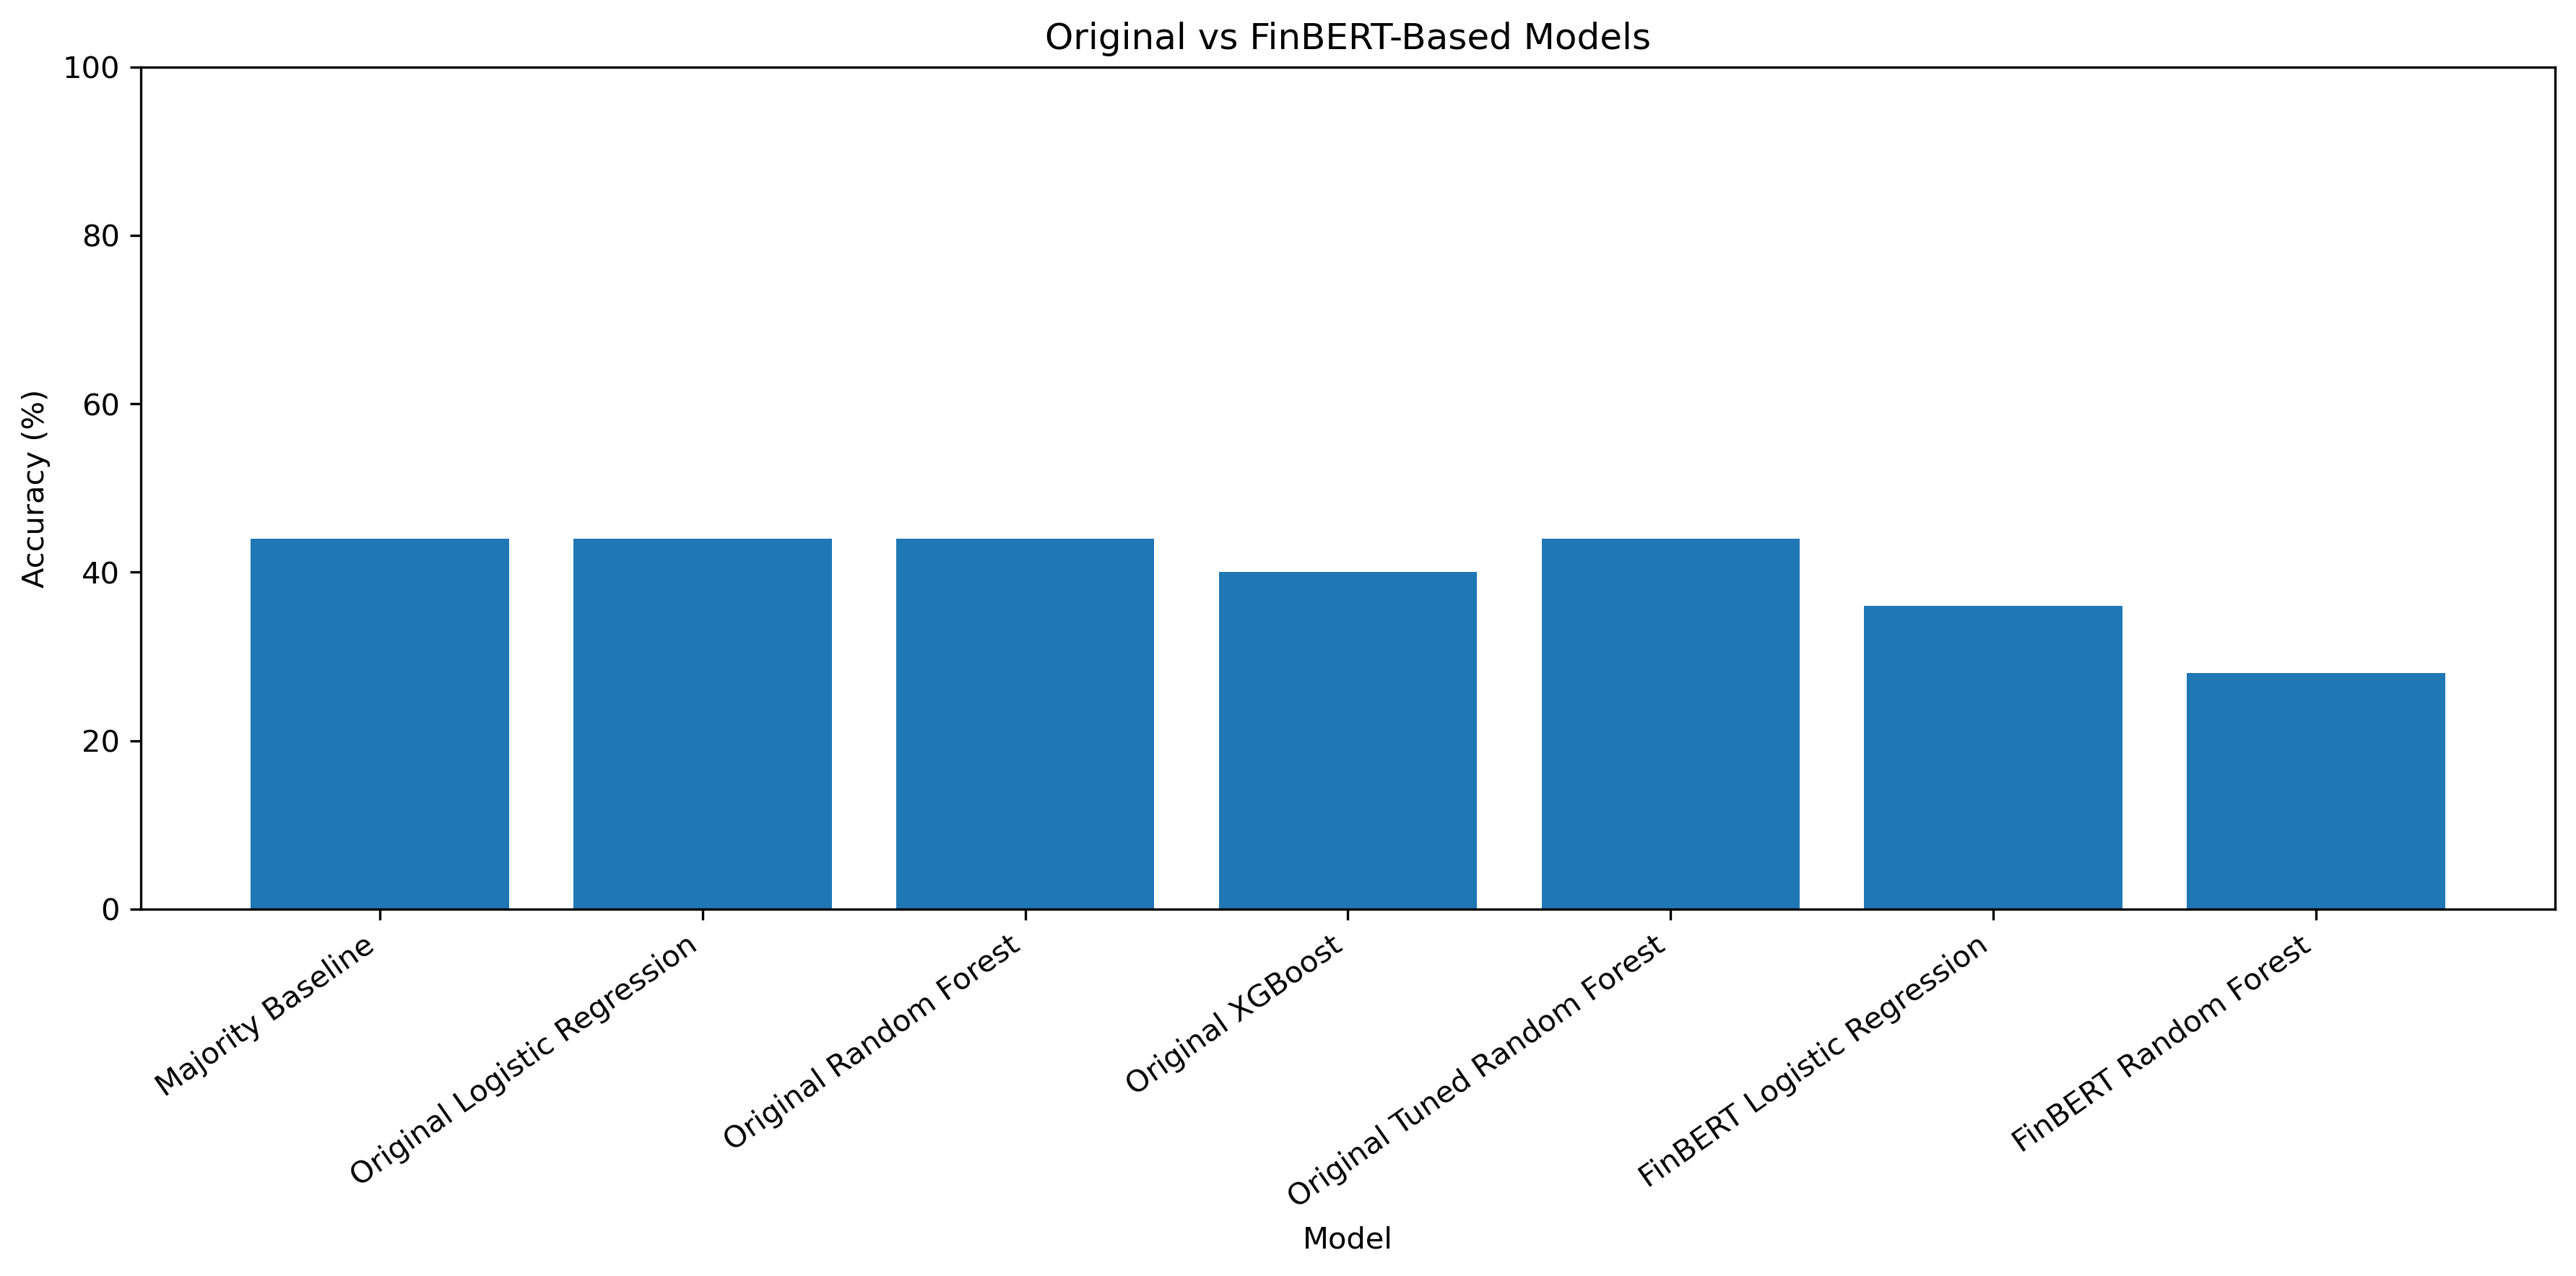
\includegraphics[
		width=0.88\linewidth
		]{../plots/original_vs_finbert_models.png}
		
		\caption{
			Final comparison of original and FinBERT-based machine-learning
			models.
		}
		
		\label{fig:modelcomparison}
	\end{figure}
	
	The most important result is that the original tuned Random Forest
	remained the strongest model on the held-out test set at 44.0\%.
	FinBERT Logistic Regression reached 36.0\%, while FinBERT Random Forest
	reached only 28.0\%.
	
	This means that the addition of FinBERT did not automatically translate
	into better next-day prediction. In this dataset, recent market
	features and the original sentiment representation were at least as
	useful as the FinBERT representation for the tested models.
	
	% ==================================================
	\section{Feature Importance}
	% ==================================================
	
	The tuned Random Forest feature importance plot provides an indication
	of which variables contributed most strongly to the model's decisions.
	
	\begin{figure}[H]
		\centering
		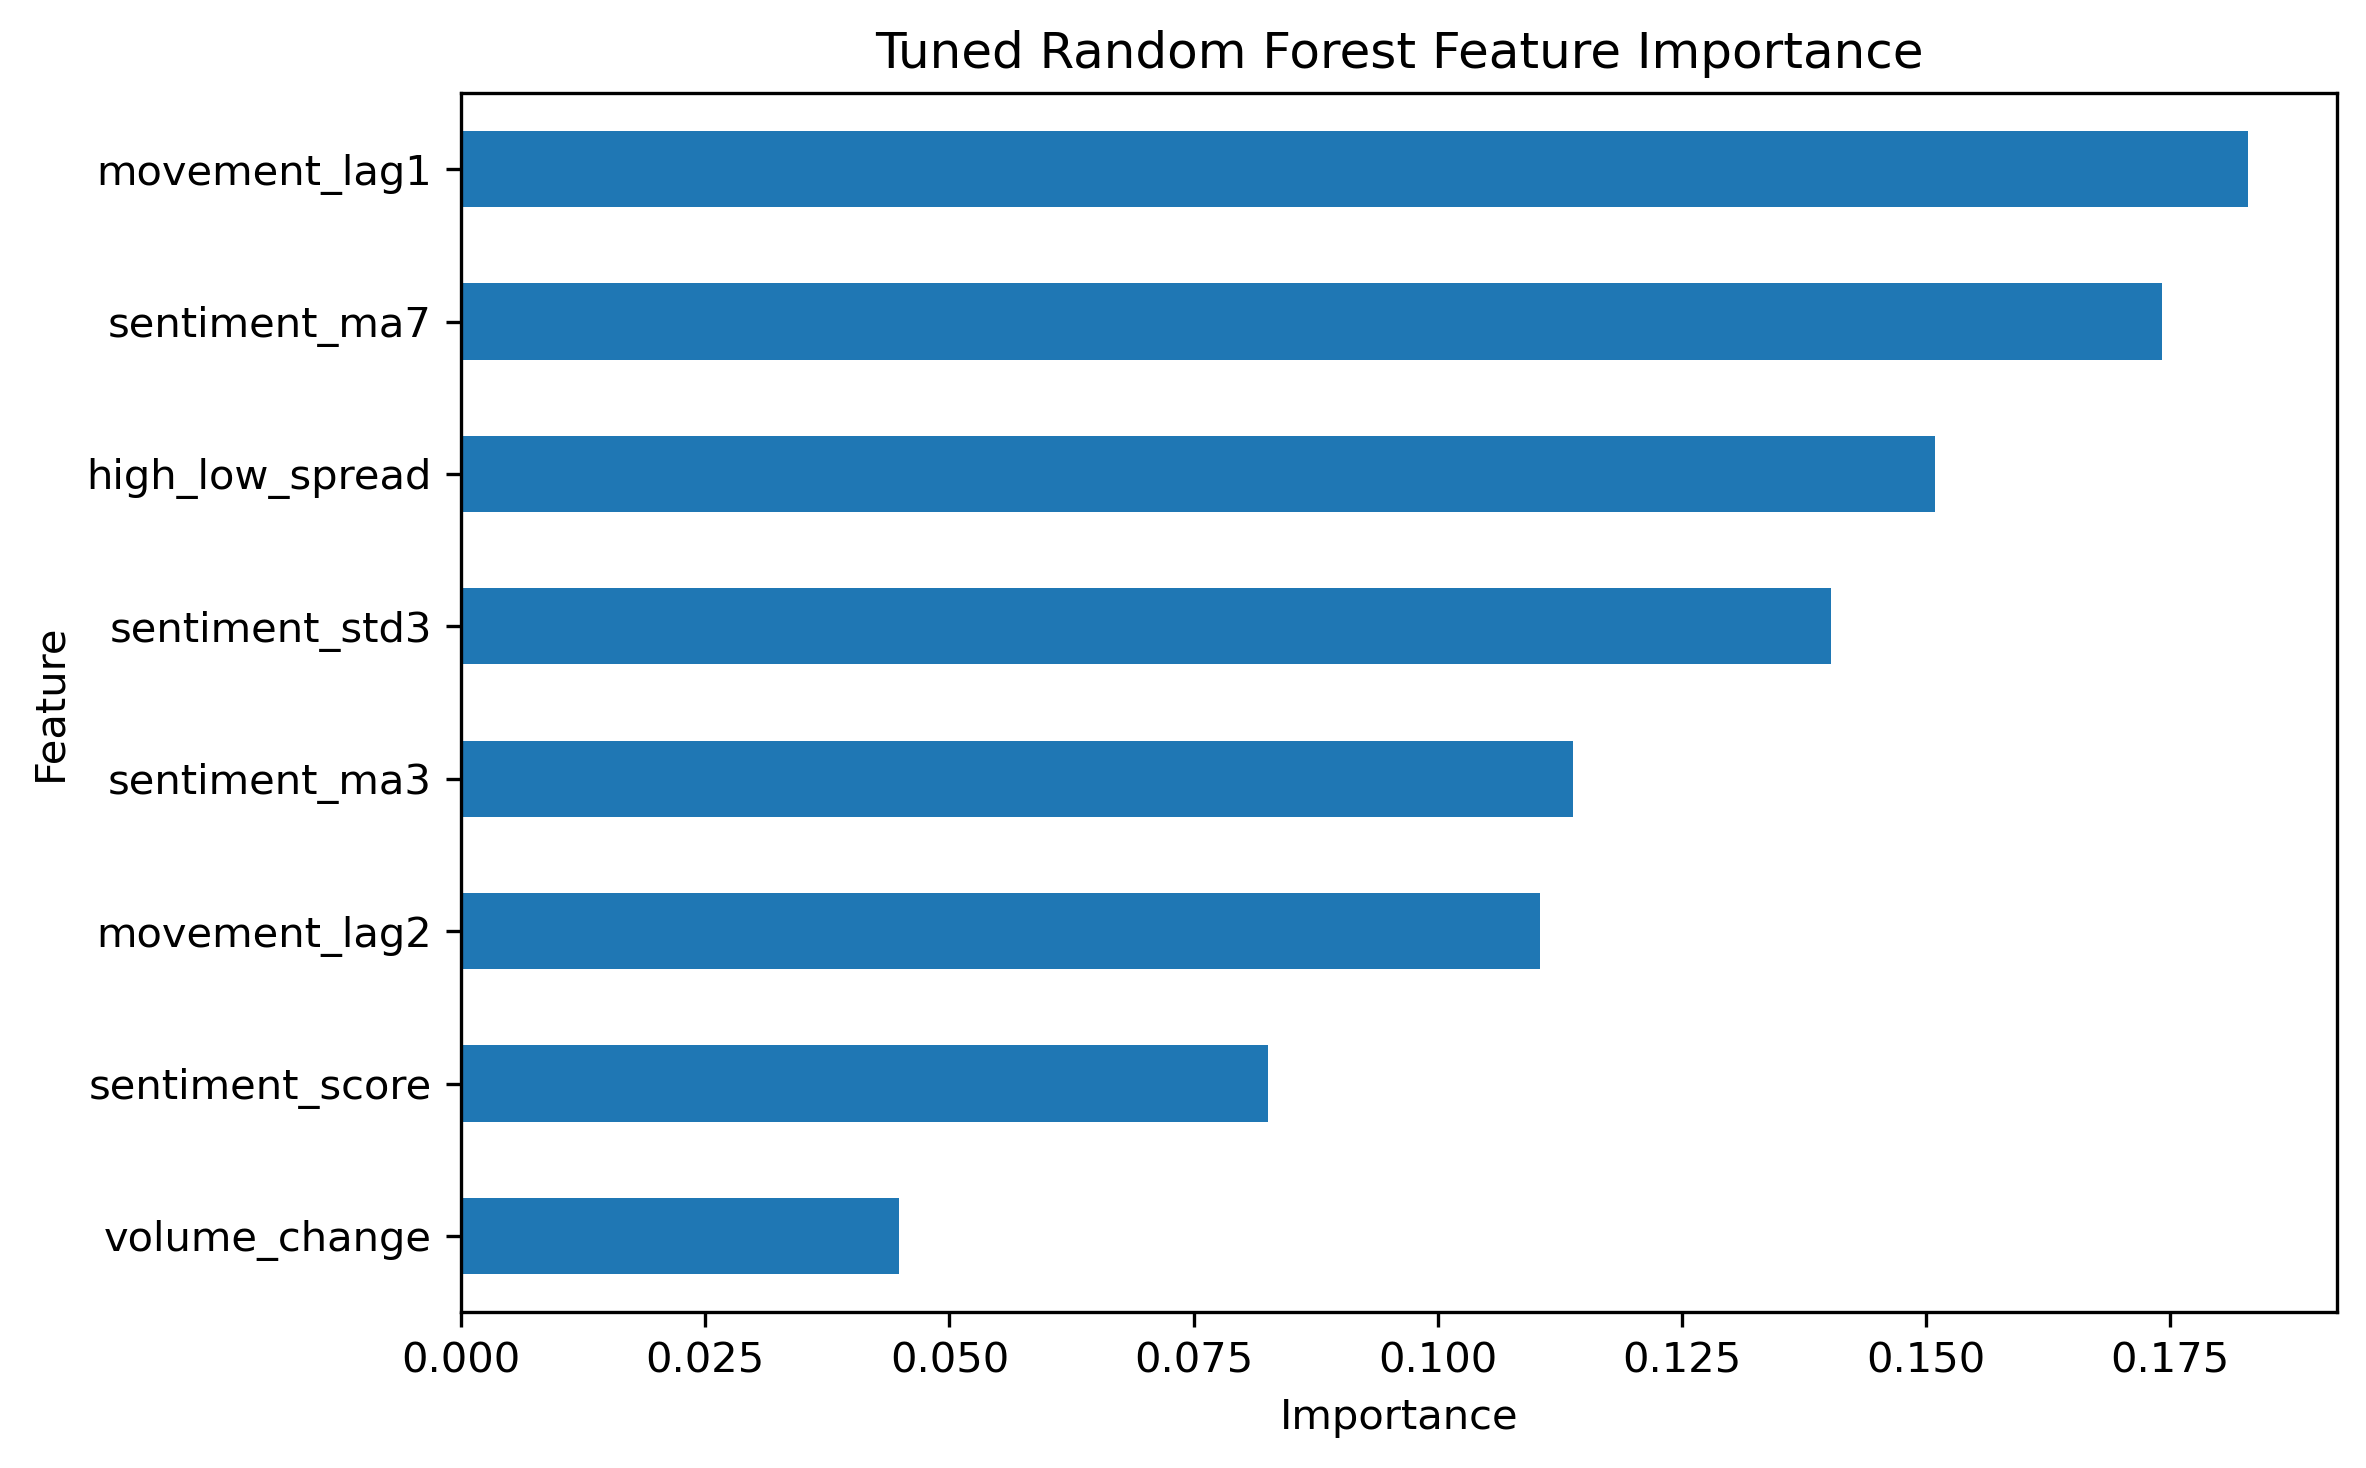
\includegraphics[
		width=0.76\linewidth
		]{../plots/tunedRandomForestFeatureImportance.png}
		
		\caption{
			Feature importance from the tuned Random Forest.
		}
		
		\label{fig:featureimportance}
	\end{figure}
	
	Previous-day market movement was among the most influential features,
	while sentiment-derived variables also contributed to the model.
	
	These results should be interpreted as model feature importance rather
	than causal evidence. A high feature-importance value does not mean
	that the feature independently causes future market movement.
	
	The results suggest that recent price behaviour contains substantial
	predictive information relative to the sentiment features in this
	small dataset.
	
	% ==================================================
	\section{Prediction Errors}
	% ==================================================
	
	The tuned Random Forest produced the following confusion matrix on the
	25-observation test period.
	
	\begin{figure}[H]
		\centering
		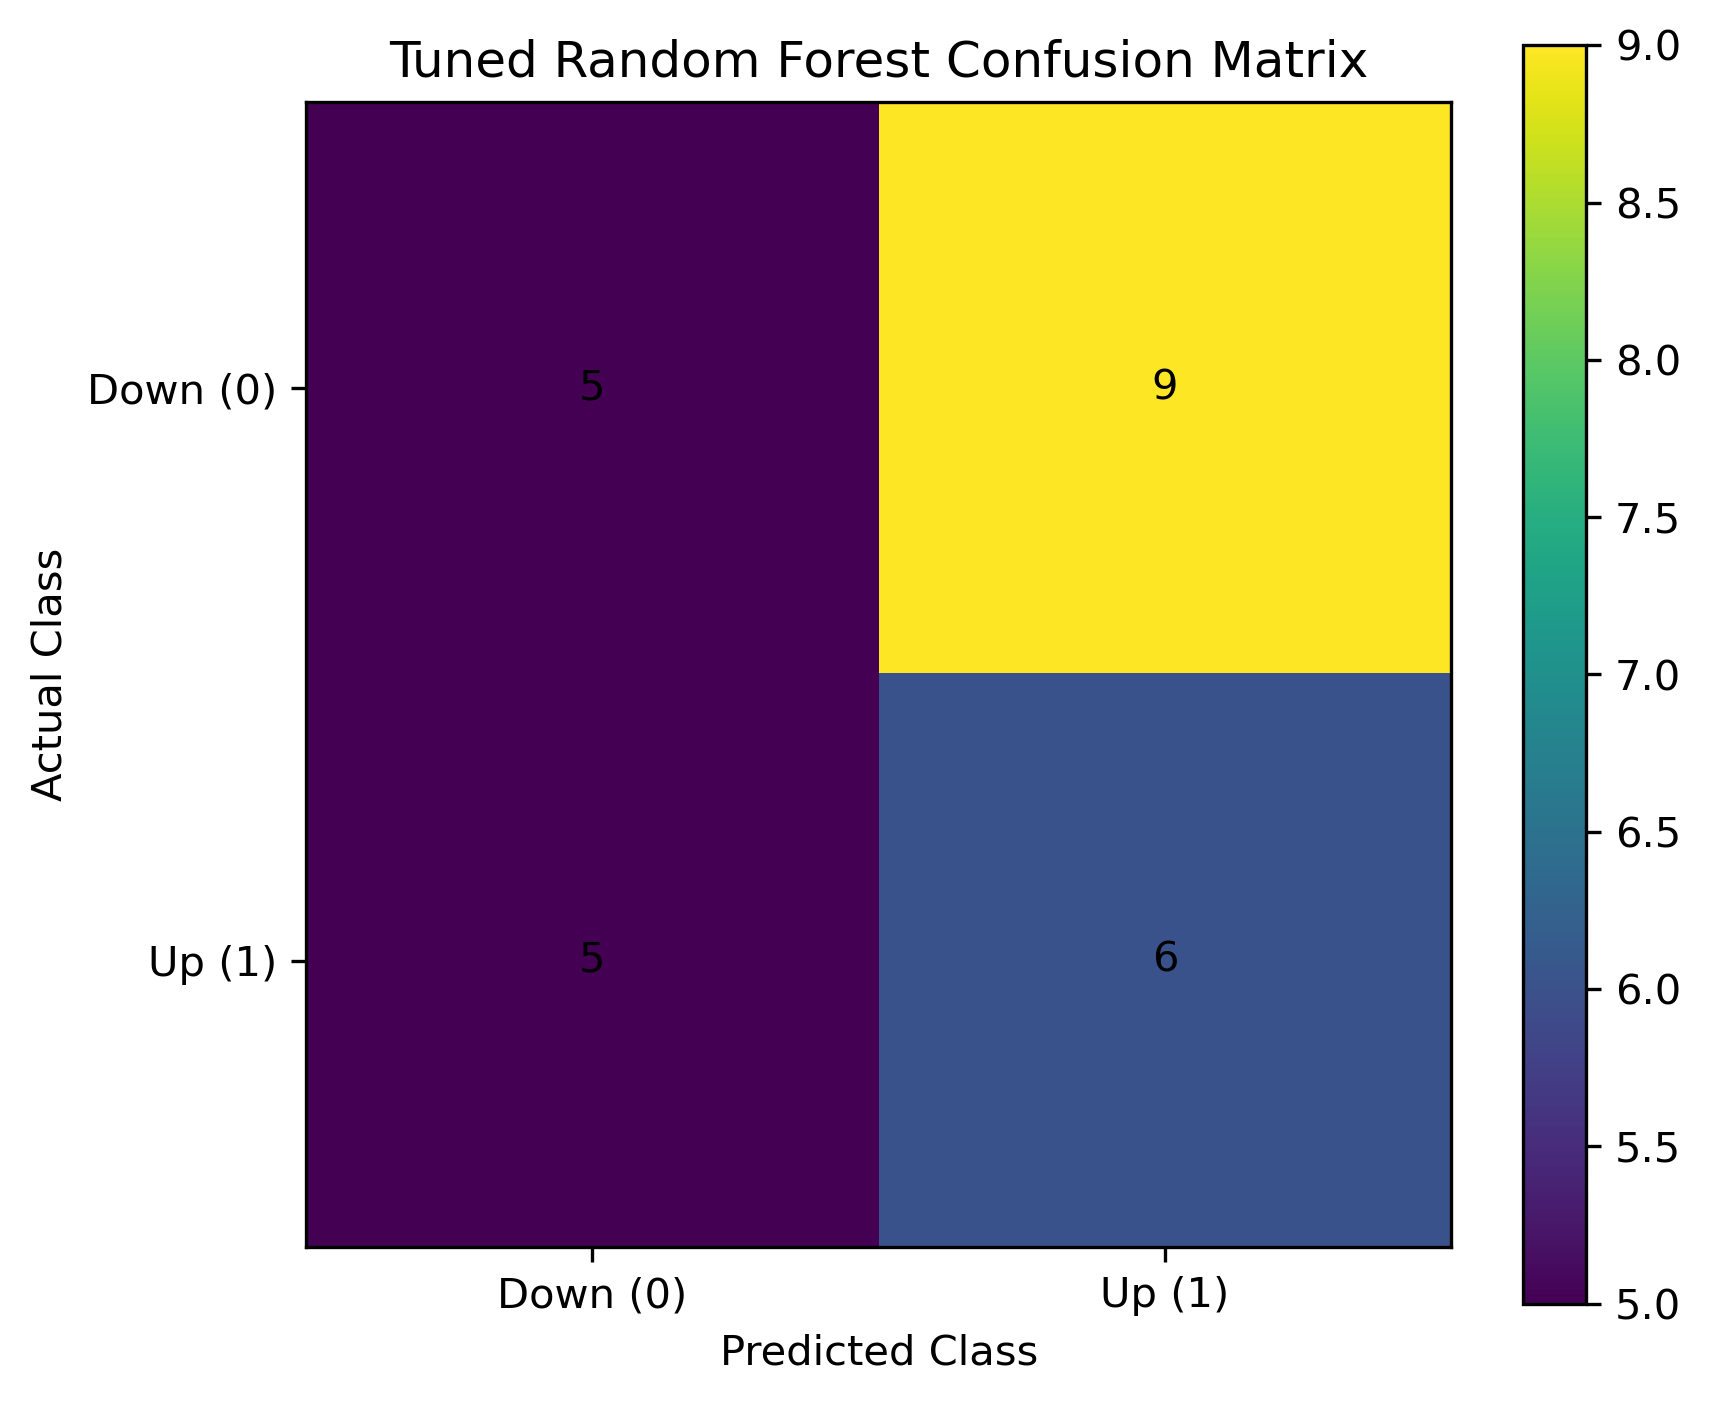
\includegraphics[
		width=0.46\linewidth
		]{../plots/tunedRandomForestConfusionMatrix.png}
		
		\caption{
			Confusion matrix for the tuned Random Forest.
		}
		
		\label{fig:confusion}
	\end{figure}
	
	The model correctly classified 5 downward movements and 6 upward
	movements, resulting in 11 correct predictions out of 25 test
	observations.
	
	Because the test set contains only 25 observations, one additional
	correct prediction changes the measured accuracy by approximately four
	percentage points. This illustrates why the reported test accuracy
	should not be treated as a highly precise estimate of long-term
	predictive performance.
	
	% ==================================================
	\section{Backtest and Discussion}
	% ==================================================
	
	A simple long-only strategy was constructed using the tuned Random
	Forest predictions. When the model predicted an upward movement, the
	strategy held the NIFTY50 for the following day; otherwise, it remained
	out of the market.
	
	\begin{figure}[H]
		\centering
		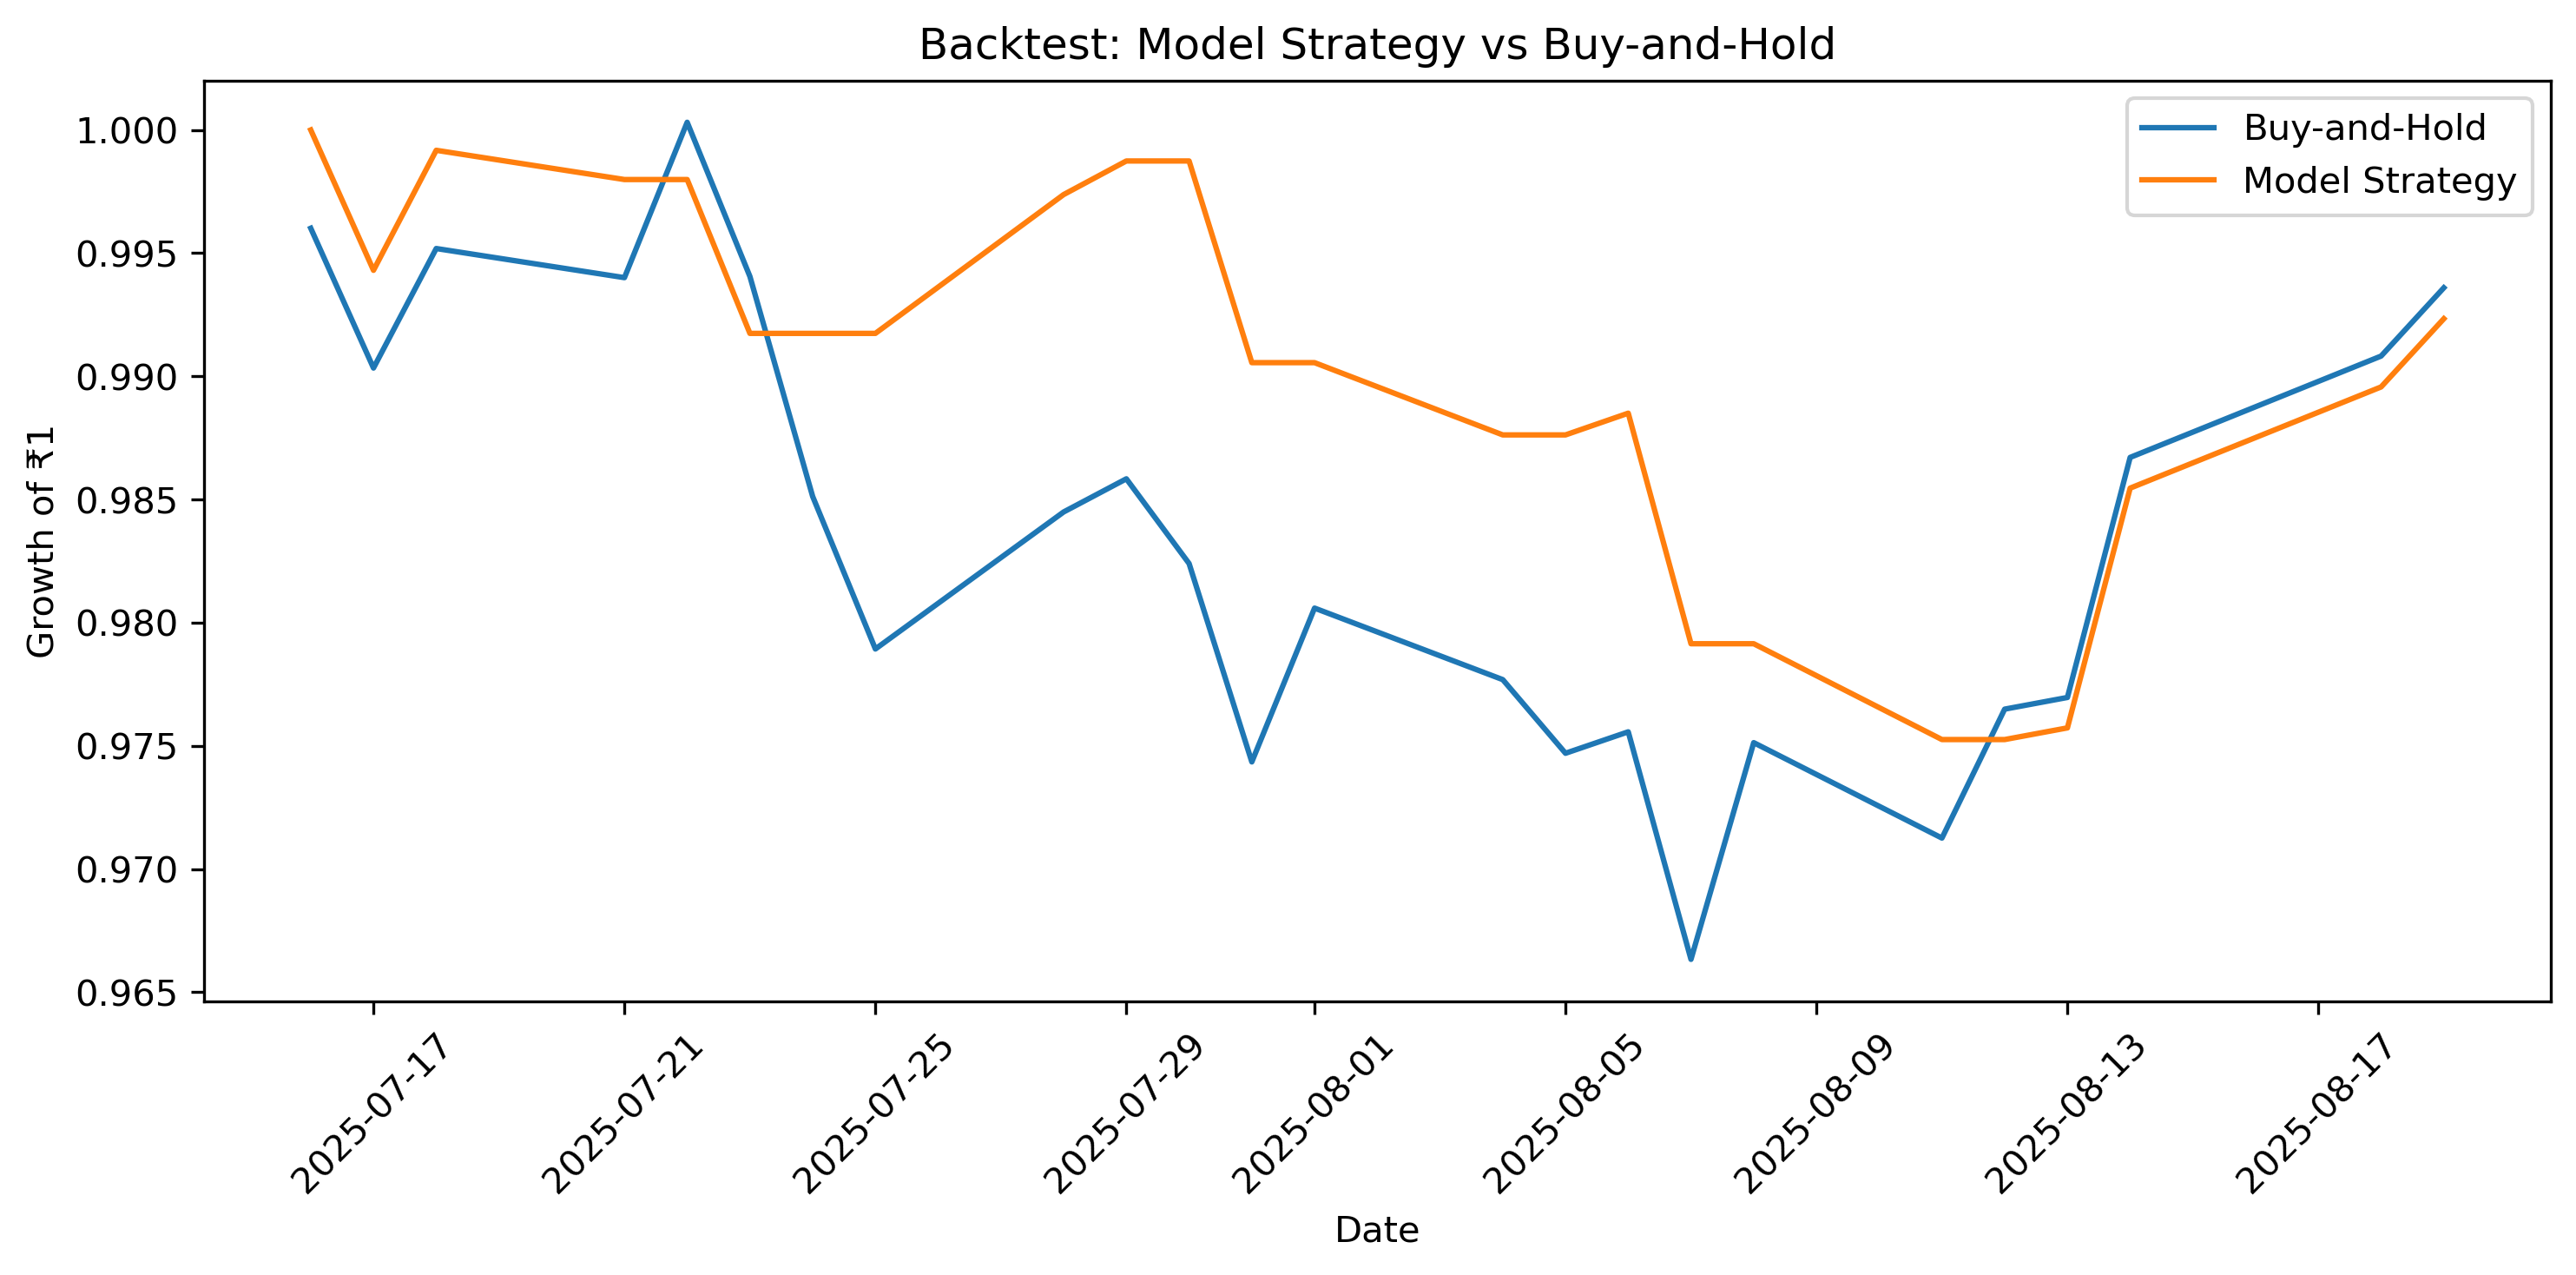
\includegraphics[
		width=0.76\linewidth
		]{../plots/backtest.png}
		
		\caption{
			Model strategy compared with buy-and-hold during the test
			period.
		}
		
		\label{fig:backtest}
	\end{figure}
	
	Over the evaluation period, the buy-and-hold strategy returned
	$-0.64\%$, while the model-based strategy returned $-0.77\%$.
	
	Therefore, the model strategy underperformed buy-and-hold by
	approximately 0.13 percentage points.
	
	The backtest is intended only as an illustrative evaluation. It does
	not include transaction costs, slippage, taxes, or other practical
	trading considerations. The small test window also means that the
	result should not be interpreted as evidence for or against a
	deployable trading strategy.
	
	% ==================================================
	\section{Discussion of the FinBERT Extension}
	% ==================================================
	
	The FinBERT extension provides an important comparison with the
	original rule-based methodology.
	
	The rule-based system is simple, transparent, and easy to interpret.
	Its score is directly determined by the occurrence of manually selected
	financial terms. FinBERT, in contrast, uses a pretrained language model
	that evaluates financial language using contextual representations.
	
	The moderate correlation of 0.407 between the two approaches indicates
	that they capture some common sentiment information while still
	producing substantially different scores.
	
	However, the machine-learning results show that a more sophisticated
	sentiment representation does not necessarily produce better
	next-day market prediction.
	
	The original tuned Random Forest achieved 44.0\%, compared with 36.0\%
	for FinBERT Logistic Regression and 28.0\% for FinBERT Random Forest.
	All of these results were obtained using the same chronological
	held-out test period.
	
	This is an important negative result rather than a failure of the
	project. It demonstrates that improving the sophistication of the NLP
	component does not automatically improve financial forecasting
	performance, particularly when the dataset is small and market
	movement is noisy.
	
	% ==================================================
	\section{Limitations}
	% ==================================================
	
	Several limitations should be considered when interpreting the results.
	
	\begin{itemize}[
		leftmargin=*,
		itemsep=1pt,
		topsep=2pt
		]
		
		\item The machine-learning dataset contains only 125 usable
		observations.
		
		\item The final test period contains only 25 observations.
		
		\item The small sample size makes the reported accuracy sensitive
		to individual predictions.
		
		\item The rule-based 59.0\% result is a same-day co-movement
		measurement and should not be interpreted as a future forecasting
		accuracy.
		
		\item The FinBERT model was used as a pretrained model rather than
		fine-tuned specifically on the NIFTY50 news dataset.
		
		\item The FinBERT sentiment features were derived from headline
		sentiment rather than full article text.
		
		\item The dataset covers a relatively short financial period.
		
		\item The backtest does not include transaction costs, slippage,
		taxes, or market-impact effects.
		
		\item Feature importance measures model dependence and should not be
		interpreted as causal relationships.
		
		\item The moderate correlation between rule-based and FinBERT
		sentiment does not imply that either method is a reliable predictor
		of future returns.
		
	\end{itemize}
	
	% ==================================================
	\section{Conclusion}
	% ==================================================
	
	The analysis investigated whether financial-news sentiment could help
	predict next-day NIFTY50 direction.
	
	The original rule-based sentiment system achieved 59.0\% accuracy when
	evaluated against the same-day target. However, this result reflects
	same-day co-movement rather than genuine future prediction.
	
	For the correctly framed next-day prediction problem, the strongest
	original model was the tuned Random Forest, which achieved 44.0\%
	accuracy on the held-out test period. This was equal to the
	majority-class baseline.
	
	The FinBERT extension produced a 36.0\% accuracy for Logistic
	Regression and 28.0\% for Random Forest. Consequently, FinBERT did not
	improve the predictive performance of the tested models.
	
	The comparison between rule-based sentiment and FinBERT produced a
	correlation of 0.407, demonstrating that the two approaches capture
	related but distinct aspects of financial-news sentiment.
	
	The backtest also showed that the model-based strategy returned
	$-0.77\%$, compared with $-0.64\%$ for buy-and-hold during the test
	period.
	
	\begin{keybox}
		\textbf{\color{Navy}Overall conclusion:}
		
		The tested sentiment representations and machine-learning models
		did not outperform the majority baseline on the held-out next-day
		prediction task. FinBERT provided a more sophisticated contextual
		sentiment representation, but it did not translate into improved
		predictive accuracy in this small dataset.
		
		Nevertheless, the project demonstrates a complete time-aware
		financial machine-learning workflow: data cleaning, sentiment
		extraction, feature engineering, next-day target construction,
		chronological evaluation, NLP model comparison, feature analysis,
		and strategy backtesting.
	\end{keybox}
	
	% ==================================================
	\section{Final Summary}
	% ==================================================
	
	The final pipeline can be summarized as:
	
	\begin{center}
		\small
		\textbf{Financial News}
		$\rightarrow$
		\textbf{Cleaning}
		$\rightarrow$
		\textbf{Date Alignment}
		$\rightarrow$
		\textbf{Rule-Based Sentiment}
		$\rightarrow$
		\textbf{FinBERT Sentiment}
		$\rightarrow$
		\textbf{Feature Engineering}
		$\rightarrow$
		\textbf{Next-Day Target}
		$\rightarrow$
		\textbf{Time-Aware ML}
		$\rightarrow$
		\textbf{Model Comparison}
		$\rightarrow$
		\textbf{Backtest}
	\end{center}
	
	The final comparison therefore answers the original research question
	conservatively: financial-news sentiment contains information related
	to market movement, but the tested sentiment and machine-learning
	approaches did not provide reliable evidence of improved next-day
	NIFTY50 prediction on the held-out period.
	
\end{document}